\documentclass[12pt,a4paper, english]{article}
% includes 
% Language setting
\usepackage[english]{babel}
\usepackage{csquotes}
\usepackage[iso]{isodate}
% Font configuration according to uni specs 
%% Calibri or Arial 11pt or Times New Roman 12pt
%\usepackage{fontspec}
%\defaultfontfeatures{Ligatures=TeX}
%\setsansfont{Calibri}
%\setmainfont{Times New Roman}
\usepackage[automark, autooneside=true]{scrlayer-scrpage}
\KOMAoptions{%
   headsepline = true,
   footsepline = true,
   plainheadsepline = true,
   plainfootsepline = true,
} 
\renewcommand\sectionmark[1]{\markright{\MakeMarkcase {\thesection\hskip .5em\relax#1}}}
\ihead*{}%\leftmark}
\ohead*{\rightmark}
\chead{}

\cfoot[]{}
\ifoot[Linus Andrae]{Linus Andrae}
\ofoot[\thepage]{\thepage}%\ of \pageref*{LastPage}]{\thepage \ of \pageref*{LastPage}}


% Set page size and margins
\usepackage[top=2cm,bottom=2cm,left=5cm,right=2cm,head=18pt]{geometry}
%% images
\usepackage{graphicx}
\usepackage{wrapfig}
\usepackage[inkscapeformat=png]{svg}
%% captions 
\usepackage{caption}
\usepackage{subcaption}
%% tables 
\usepackage{booktabs}
%% maths
\usepackage{amsmath}
%% colors
\usepackage{xcolor}
%% links and refs and citations 
\usepackage{setspace}
\usepackage[colorlinks=true, allcolors=black]{hyperref}
\usepackage[capitalize]{cleveref}
\usepackage[backend=biber, style=authoryear]{biblatex}
%% acronyms and glossary 
%\usepackage[acronym,]{glossaries} 
\usepackage[automake,acronym,postdot,stylemods,translate=babel]{glossaries-extra}
% varwidth
\usepackage{varwidth}
%% include code snippets
\usepackage{listings}
%% Kerning
\usepackage[protrusion=true,expansion]{microtype}
%% Tikz
\usepackage{tikz}
\usetikzlibrary{shapes.geometric, arrows, backgrounds, automata, positioning}
%% Some diagram definitions
  %
\tikzstyle{startstop} = [rectangle, rounded corners, minimum width=3cm, minimum height=1cm,text centered, draw=black, fill=red!30]
\tikzstyle{io} = [trapezium, trapezium left angle=70, trapezium right angle=110, minimum width=3cm, minimum height=1cm, text centered, draw=black, fill=blue!30]
\tikzstyle{process} = [rectangle, minimum width=3cm, minimum height=1cm, text centered, draw=black, fill=orange!30]
\tikzstyle{decision} = [diamond, minimum width=3cm, minimum height=1cm, text centered, draw=black, fill=green!30]
\tikzstyle{arrow} = [thick,->, > = stealth]

\usepackage[version=4]{mhchem} % for chemical reaction formulas
%% title page
\usepackage{titling} % for cooler titlepages 
% configuration 
\bibliography{refs.bib} % Entries are in the refs.bib file
% configure python code snippets
\lstdefinestyle{PyStyle}{%
    commentstyle=\color{olive},
    keywordstyle=\color{magenta},
    numberstyle=\tiny\color{gray},
    stringstyle=\color{purple},
    basicstyle=\footnotesize,
    breakatwhitespace=false,         
    breaklines=true,                 
    captionpos=b,                    
    keepspaces=true,                 
    numbers=left,                    
    numbersep=5pt,                  
    showspaces=false,                
    showstringspaces=false,
    showtabs=false,                  
    tabsize=2,
    language=python
}
\date{\today}
% setup title 
\title{\textbf{\huge Impact of Climate and \\Land Cover Change \\in Urban Heat Islands}}
\author{%
\begin{tabular}{ll}
Supervisor: &Prof.\ Dr.\ Annette Ladstätter-Weißenmayer\\
Secondary Supervisor: &Dr.\ Adrian Fessel\\ 
Submission Date:\ &30.04.2024\\
\ &\ \\
\ &\ \\
\ &\ \\
\ &\ \\
Linus Andrae &  \\%
Hegelstraße 24& \\ 
28201 Bremen&  \\
Matriculation Number: & 6015384 \hfill\\
Current Date:&\thedate\\
\end{tabular}
}%

\makeglossaries%
\setabbreviationstyle[acronym]{long-short}
% Acros
\newacronym{USGS} {USGS} {United States Geological Survey}
\newacronym{LST}  {LST}  {Land Surface Temperature}
\newacronym{LULC} {LULC} {Land Use/ Land Cover}
\newacronym{UHI}  {UHI}  {Urban Heat Island}
\newacronym{SUHI} {SUHI} {Surface Urban Heat Island}
\newacronym{NDVI} {NDVI} {Normalized Differential Vegetation Index}
\newacronym{HI}   {HI}   {Heat Index}
\newacronym{NIR}  {NIR}  {Near Infrared}
\newacronym{OSM}  {OSM}  {Open Street Map}
\newacronym{TOA}  {TOA}  {Top of Atmosphere}
\newacronym{VOC}  {VOC}  {Volatile Organic Compounds}
\newacronym{ML}   {ML}   {Machine Learning}
\newacronym{SVM}  {SVM}  {Support Vector Machine}
\newacronym{ECMWF}{ECMWF}{European Center for Medium-Range Weather Forcasts}
\newacronym{WBGT} {WBGT} {Wet Bulb Globe Temperature}


\newglossaryentry{dilated}%
{%
  name={Dilation},
  description={An image processing operation that extends objects by adding pixel to the outside of an object}
}
\newglossaryentry{eroded}%
{%
  name={Erosion},
  description={An image processing operation that reduces the size of objects by removing pixels at the border of the object}
}
\newglossaryentry{lib}%
{%
  name={Library},
  description={a bundled collection of resources (e.g.\ algorithm) to be ease software development}
}

\newglossaryentry{DWD}%
{%
name = {Deutscher Wetter Dienst},
description= {German Meterological Service, the german meterological society}
}

\newglossaryentry{sentinel3}%
{%
  name={Sentinel-3},
  description={A Pair of Satellites, that are part of the Copernicus constellation. Using 21 spectral channels with a resolution of 300~m per pixel}
}
\begin{document}
  \begin{titlingpage} %This starts the title page
\pagenumbering{Alph}
\thispagestyle{empty} 
\begin{center}
\begin{large}
  \textit{University Bremen}\\
\end{large}
\vspace{4cm} %You can control the vertical distance
\begin{large} 
\textbf{\thetitle} 
\end{large}
\theauthor\\
\thedate\\
\vspace{13cm} %Put the distance you need.


\includegraphics[width=0.3\textwidth]{img/res/uniLogoIUP.png}
\hspace{4cm}

\includegraphics[width=0.3\textwidth]{img/res/logo_ohb_digital.png}

\end{center}
\end{titlingpage}
\pagenumbering{arabic}

  \newpage

  \begin{abstract}
\noindent
Urban Heat Islands (\acp{UHI}) pose a growing health risk by exacerbating heat stress for residents of urban areas. 
Due to the increased prevalence of extreme weather events and heat waves and as a cause for higher energy consumption, \acp{UHI} become more relevant as a topic for city planners and policy makers to consider.
Identification of areas most impacted or at risk require a data backed tool set to aid urban planning. 
This study presents a comprehensive pipeline developed using Python to automate the processing and analysis of Landsat 7,8 and 9 remote sensing imagery.
The pipeline facilitates the generation of Normalized Difference Vegetation Index (NDVI) and heat maps, running statistical analysis of factors known to create \acp{UHI} of a provided area of interest, serving as a robust toolset for the investigation and detection of \acp{UHI}.
The methodology employed leverages the spectral characteristics of Landsat data to provide high-resolution insights into temperature variations within urban areas as well as statistical analysis of the composition of the identified Urban Heat Islands.
The ultimate aim is to offer actionable guidance to city planners and developers for the mitigation of \acp{UHI}, by classification of \acp{UHI} on different scales.
At the current implementation level the pipeline is able to detect \acp{UHI} from level one brightness temperature and the statistical analysis indicate a strong correlation between land cover types and heat island intensity, affirming the utility of the pipeline in urban climate studies.
%To analyse and identify Urban Heat Islands using remote sensing imagery
\end{abstract}

  \newpage

  \tableofcontents
  \listoffigures
  \listoftables
  \newpage
  % Abbreviations first
  %\printglossary[title=Abbreviations, type=abbreviations]
  \printglossary[title=Acronyms, type=acronym]
  %then the main glossary
  \printglossary%
\newpage
\onehalfspacing%

\section{Introduction}\label{sec:intro}
\subsection{A historical introduction of urban heat island research}
  The scientific investigation of the urban climate and the influence of human settlements and activity on the local atmosphere and temperature has been studied for more then 200 years.%
  \cite{Howard1833}~investigated the climate of London in a study from 1819 to 1827 and a similar study was conducted in Paris in the 1850s by~\cite{renou1862differences}.%
  The first mobile measurement campaigns around the topic of urban climate were conducted by~\cite{peppler1929auto} and~\cite{tollner1932untersuchungen} and investigated the spacial distribution of temperatures within urban areas  in the 1920s in Germany and Austria. 
  This type of measurmenet were repeated in multiple cities around the globe at the time.\\
  The term Urban Heat Island was coined in the 1960s in publications regarding case studies in London~\cite{Chandler1961} and Montreal~\cite{Oke1968}. % TODO there was a paper claiming otherwise
  During this time the influences and understanding of the interaction between the human industrial activity, the land change by urbanisation and industrialization and the influence thereof on temperatures and pollution was investigated by numerous case studies using fixed or mobile weather stations.
  Often health problems within industrial areas or incidence like the 1930 meuse valley fog catastrophe, in which exhaust gases, including fluorine gas, combined with an inversion weather condition, forming a cloud over the area causing the death of at least 60 people.
  The \textit{great smog} in 1952 in London and the meuse valley fog triggered an scientific intrest in the interaction between human settlement, pollution and meterological phenomena on human health and the environment, shaping the idea of an urban climate.\\ \\ 
  To understand the urban meterology the first use of helicopters and air planes to measure vertical temperature profiles were documented in the 1950s  
  %TODO add source 
  All these studies focused on the atmospheric heat distribution over urban areas and resulted in the development of physical energy transport models for these. 
  These models required a deeper understanding of the surface properties and the temperature distribution within the urban area.\\ \\
  % 
  Then newly available remote sensing devices such as infrared imagers made it possible to observe the urban environment from above and detect temperature hot spots using airborne and satellite images.  
  %  
  First investigations regarding the feasibility of this approach were proposed in the late 70s (\cite{Watson1975},~\cite{Carlson1977} and~\cite{Block1978}) but the resolution of satellite images insufficient for detailed investigations of Urban Heat Islands.\\
  A first study using satellite infrared imagery were conducted in 1978 using the NOAA 5 Satellite (with a spacial resolution of 1km)\cite{Matson1978}. 
  Multiple studies in the 70s and 80s used images taken from planes or helicopters to aid the investigation of smaller scale effects within the urban surface temperature distribution (e.g.~\cite{Landsberg1979},~\cite{ljungberg1980use} and~\cite{Foster1981}).
  With advances in satellite technology the resolution and data availability increased. 
  The Landsat program stared in 1975 and since \textit{Landsat 4} was launched in 1982 the Landsat program continuously provides thermal infrared data of the whole planet. 
  The increased resolution that allows pixel sizes between 60 m (\textit{Landsat 7}) and 120 m (\textit{Landsat 4} and \textit{Landsat 5}), allows investigation of smaller patterns within urban areas.\\
  Increased revisit frequency of roughly two weeks made remote satellite data a more useful and widely used tool in the research of urban meteorology and urban heat islands. 
% Add the 2008 - 2010
  Over the past 30 years, the amount of available remote sensing data skyrocketed, Landsat 8 and 9 produced over 6 million images since the start of operation in 2013. \Cref{fig:landsatproductsovertime} shows the number of scenes taken by the Landsat satellites alone per year.
  \begin{figure}[!htbp]
    \centering
    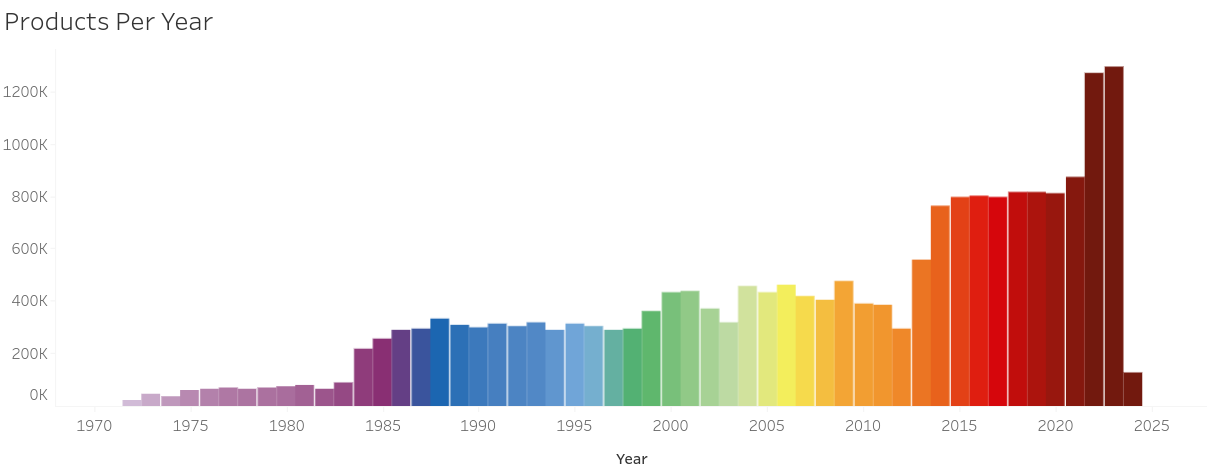
\includegraphics[width=\textwidth]{img/LandsatDataArchiveStatsProductsPerYear.png}
    \caption{Number of Landsat Products per year over time (as of Feb.2024) by the~\cite{landsatstats}\label{fig:landsatproductsovertime}}
  \end{figure}
  The rise in availability on the one hand makes it easier for researchers and companies to use the data, but requires increased computing and storage availability, to manage the increased data amount.
  This offers the possibility of creating scientific studies covering a wide range of cities over time, using the same sensor and tools. 
  \Cite{Sobrino2020} suggested a methodology to compare \glspl{UHI} using \gls{sentinel3} images and conducted a broad study of \glspl{UHI} severity in cities around the world. 
  Over the past years the number of scientific papers investigating the issue from multiple angles increased significantly (ct. \cite[P. 3]{Piracha2022b}).
In conclusion, the advancement of remote sensing technology, particularly the availability of infrared imagers and satellite imagery, has revolutionized the study of urban heat islands. 
From the early investigations and roots of the field in meterology and public health the research field expanded touching urban development, climate science, atmospheric chemistry and medicine as well as social sciences.
The scope of studies from case studies conducted in the 70s to the current abundance of data provided by satellites like Landsat 8 and 9, researchers now have the tools to analyze urban surface temperature distribution with unprecedented detail and accuracy.
The increase in data availability has not only facilitated research on urban meteorology and heat islands but has also presented new challenges in terms of data management and analysis.
Despite these challenges, the potential for conducting comprehensive studies across various cities using consistent sensors and methodologies is now within reach.
%As demonstrated by studies such as the one conducted by \cite{Sobrino2020} using Sentinel-3 images, the future of urban heat island research holds promise for gaining deeper insights into the impacts of urbanization on local climate patterns worldwide.
% TODO more and finish
The next step in advancing the comprehension of \glspl{UHI} involves gaining a deeper understanding of how various parameters contribute to the formation and intensity of \glspl{UHI}.
With the widespread introduction of countermeasures to \glspl{UHI} and climate change resilience techniques in different cities, continuous monitoring of statistical parameters and indices becomes more relevant in order to assess the effectiveness of the mitigation strategies. 

\subsection{Research Question}
In this thesis, the impacts of land cover changes, such as urbanisation, and rising average temperatures on the urban heat island (UHI) phenomena are investigated.
The specific questions posed are:
\begin{itemize}
    \item What is the influence of urbanisation on the size of urban heat islands?
    \item How significant is the impact of urbanisation on UHI, both in terms of absolute and relative temperature changes?
    \item What is the effect of rising average temperatures on the UHI effect?
    \item Is it feasible to model UHIs using the identified impacts of temperature and land use change?
\end{itemize}

\subsection{Methodology}
To address the outlined research questions, the following methodology is employed:
\begin{enumerate}
    \item Utilisation of multi-spectral visible and thermal infrared satellite data for Surface Urban Heat Island (SUHI) measurements.
    \item Application of machine learning algorithms to create time series of land use and land cover (LULC) for selected cities. % TODO add cref to section with cities
    \item Longitudinal measurement of UHI intensity over time.
    \item Projection of UHI development based on the findings from \gls{SUHI} measurements and \gls{LULC} analysis.
    \item Use of various indices to measure heat stress and other parameters for assessing UHI intensity.
    \item Provision of an outlook on further research directions in the field of UHI phenomena.
\end{enumerate}

  \subsection{Structure of the Thesis}
    In the introduction as well as \cref{sec:background} previous work and an overview of the current understanding of the urban heat island effect and research in this area is accessed. 
  %comparable definition
    \Cref{sec:definition} explains the used adaptation of the proposed methodology by~\cite{Sobrino2020} to create a definition of surface urban heat islands that is usable for comparing \glspl{UHI} in different cities.  
    \Cref{sec:LULC} explains how the measurements  and investigations of the impact of land use and land cover changes by build up where done.
    In \Cref{sec:UHITempImp} the impact of changing temperatures an increase of extreme weather phenomena on the intensity and seasonal variety of \glspl{UHI} was investigated. 
    After these the \cref{sec:conclusion} combines the findings of the previous chapters, shows what other investigations should be investigated further and where the research could be improved. 
%
%
\section{Background}\label{sec:background}
%\section*{Acknowledgements}
\subsection{Urban Heat Islands}
%
Due to increase in global temperature as well as increased occurrence of extreme weather and periods of heatwaves, this phenomenon will likely increase in intensity and will also occur in cities at higher latitudes~\cite{Sachindra2016}\cite[p.~904]{Wilby2008}.
\glspl{UHI} are a spacial phenomenon that occurs on different scales and intensities, this makes observation using remote sensing data a good and widely used approach~\cite{Weng2003}.\\
\glspl{UHI} are distinguished into surface and atmospheric \glspl{UHI} as discussed in the sections below. 
Since the phenomenon is known for a long time, mitigation strategies have been proposed to reduce the impact on well-being and intensity of the UHIs.
%
\subsubsection{Surface Urban Heat Islands}\label{sec:suhi}
\glspl{SUHI} are areas of higher surface temperatures within urban areas compared to rural areas due to the materials used and heat from mobility, electrical appliances, heating and cooling as well as less vegetation and higher sealed surfaces that reduce surface water availability\cite[pp. 7-12]{EPA2008}. 
The \glspl{SUHI} are a small scale phenomenon that has a high seasonal variability and is most intense in summer.
%
\subsubsection{Atmospheric Urban Heat Islands}\label{sec:at_uhi}
Atmospheric \glspl{UHI} is the increased air temperature within an urban area. 
This are more dependent on weather and local topology and are in part caused by the slower cooling rate of build up land causing responsible for \glspl{SUHI}.
%Under certain conditions the increased temperature will form a hot air pocket, that will trap the head and reduce airflow from and to the area. \\
The main factors in forming urban heat islands is the thermal storage capacity of materials used in urban areas like concrete, asphalt and steel, that have a high heat capacity and heat up quickly during the day and emit the stored thermal energy as sensible heat with a delay (eg.~during the night)\cite{Ramamurthy2014}. 
High surface sealing and lack of vegetation reduce surface water availability and diminish evaporation and the cooling effect of latent heat causing more thermal energy to be available as sensible heat. %todo source (sailor?  or first source)
Another factor is the heat produced by human activity such as industrial processes and combustion engines.
As a consequence of higher temperatures, active cooling devices are more frequently used for buildings and vehicles. 
The emitted thermal energy of these heat pumps further increases the surrounding temperature, reinforcing the effect.
\\
There are multiple adverse effects and possible mitigation techniques for the reduction of atmospheric urban heat islands (e.g. \cite{Nichol1994} and \cite{Stewart2011}). % list studies.  . 
%The city climate has been studied extensively since the 1870s
Advective cooling can be observed when the temperature gradient generated airflow from the cooler surrounding areas towards the hot areas within the city, cooling it down\cite{HaegerEugensson1999}. \\
Urban areas with no close water body (generating sea breezes as well as latent heat transport) and with lower average wind speed are more likely to be affected by urban heat islands\cite{Ramamurthy2017}. 
Higher temperatures due to \glspl{UHI} cause stress to animals and humans increasing health risk due to heat stroke and increased surface level ozone concentration~\cite{Santamouris2020}.
%
\newpage
\subsubsection{Pollution and Urban Heat Islands}
\begin{wrapfigure}{r}{0.5\textwidth}
  \begin{center}
    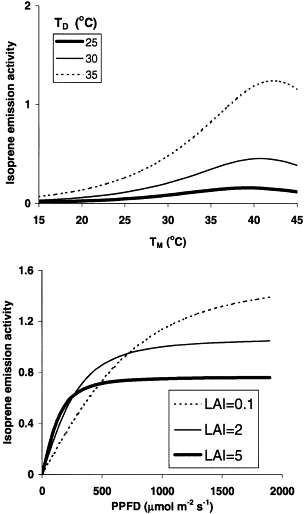
\includegraphics[width=0.48\textwidth]{img/VOCsGraphs}
  \end{center}
  \caption{Temperature dependence of isoprene emmision of 15 minute ($T_M$) and 15 day ($T_D$) mean temperature from \cite{Guenther2000}}\label{fig:tempVOC}
  % TODO add copyright note (with regards to this figure)
\end{wrapfigure}
Air pollution has been a documented problem for the quality of life since the start of the industrialisation. 
While in the 19th and first halve of the 20th century the major problem came from unfiltered exhaust of the burning of coal and wood for heating and haevy industy.
The major pollutants in urban areas in the 21st come from car exhaust and by products of industrial Agricultural. %TODO sources 
\\
One major health concern comes from tropospheric ozone, that is created in photochemical reactants of primary pollutants such as NOx compounds that are created as a byprocduct of fossile fuel burning. 
Another source of tropospheric ozone ist the photochemical reaction of \glspl{VOC}, that are mainly of natural origin~\cite{Kansal2009}.
Trees release VOCs like isoprene and terpenes as a protective mechanism against temperature stress and to protect from insects and pests, this gives the \glspl{VOC}
a high seasonal variability. 
With rising global temperatures the number of days with temperatures causing heat stress in trees (e.g.\ with a temperatur above 30 °C shown in \cref{fig:tempVOC}) has been increasing (see \cref{fig:ubaTemp}).%TODO change picture to italy or some region with higher temperatures
Due to the effect of Urban heat islands that causes a further increase in temperature within urban areas,  there is an expected increase of tropospheric ozone due to \glspl{VOC} and higher reaction rates in densly populated areas with higher mortality and other health consequences (s.~\cite{Ebi2008}).\\
\begin{figure}[!htbp]
  \begin{center}
    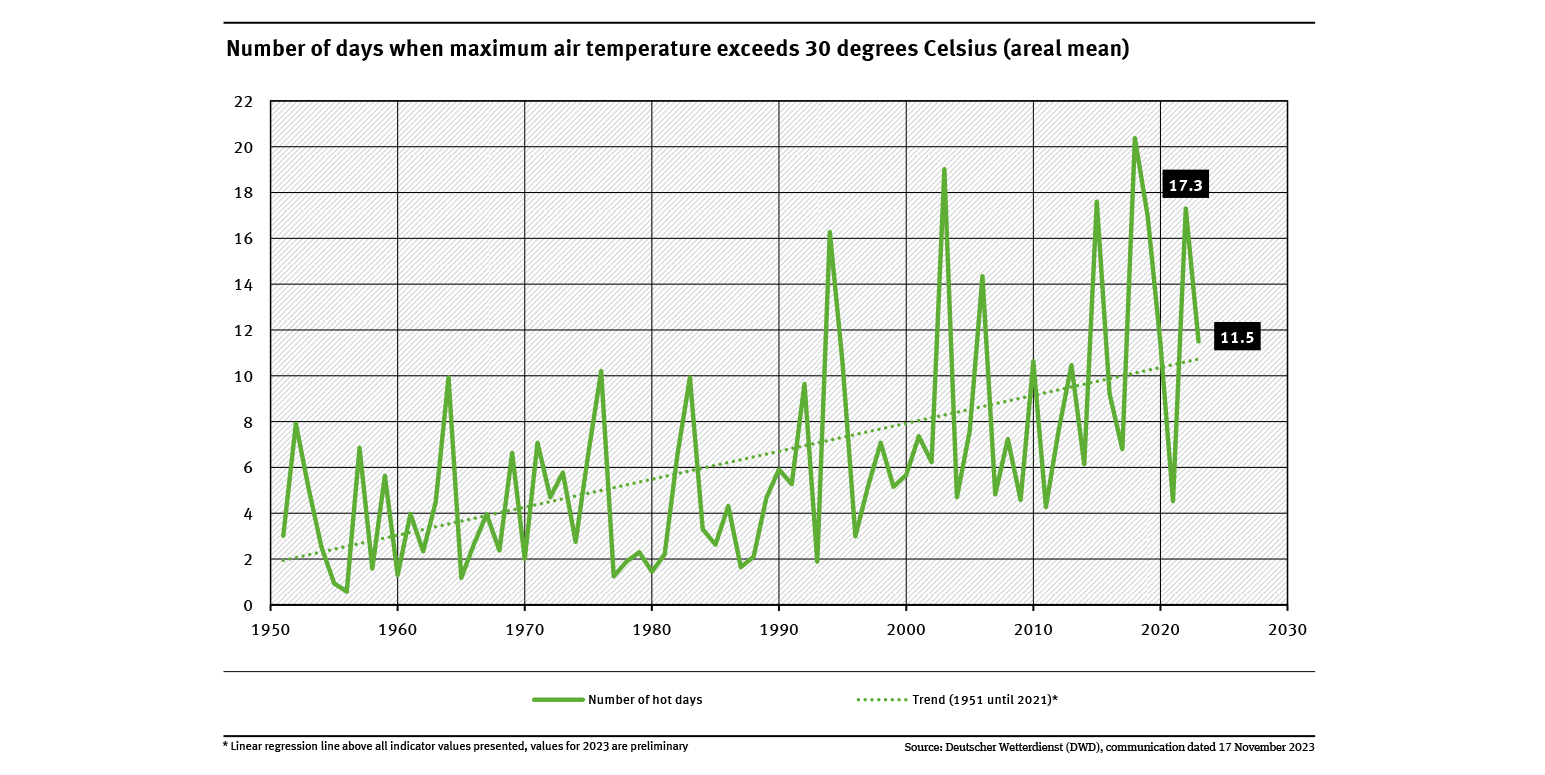
\includegraphics[width=\textwidth]{img/ubaTemp}
    \caption{Number of days with maximum Temperatures above 30°C in Germany~\cite{uba}\label{fig:ubaTemp}}
  \end{center}
\end{figure}

\subsubsection{Mitigation techniques for Urban Heat Islands}
The idea to reduce the urban heat buildup and health problems in cities has been done before the topic was studied. 
In hot areas around the globe different methods where used to create spaces with cooler temperatures for rest and work. 
All over the meditareiean houses are painted white to increase reflection of sunlight. 
In newer studies this traditional painting pattern has shown to be an efficient counter to high solar intensities ( \cite{Fayad2021}).
% Many cultures use passive cooling  roofs TODO find paper also passive ventilation and such 
Another method of larger scale cooling is the increase of vegetation to increase latent heat transport and water availability.
Green roof concepts, green facades, parks or street trees all show effective in reducing temperatures within the urban environment (see~\cite{Ramamurthy2014},~\cite{Feyisa2014},~\cite{Dimoudi2003} and~\cite{Gartland2008}).


\subsection{Land Surface Temperature}
Land surface temperature is the temperature at which an object emits infrared radiation according to plank's law\cite{Liang2020}.
Using remote sensing methods this quantity can not be directly observed since the satellite is observing \gls{TOA} brightness temperature.
This temperature can be transformed to a \gls{LST} using atmospheric correction and correction for the emissivity of the ground.
The conversion factor is data source dependent and can be found in \cref{sec:lstcalc}.

%
\subsection{Air Temperature}
Urban heat islands that impact human health are the atmospheric urban heat islands. 
These are defined by the air temperature of the urban area and the air temperature outside that area. %todo fix a bit 
%
During the day the air temperature is lower then the surface temperature\cite{EPA2008}, during the night the hot surfaces radiate off the energy heating the surrounding air.\\
%
There are multiple factors impacting urban air temperature. 
Combustion from traffic and industrial processes, produce heat as a by product that heats the surrounding air. 
HVAC systems also produce heat, when cooling buildings. This further increases the air temperature increasing cooling need within the urban area. 
    \subsection{Indices}
Many different indices are used for analysis of images or parameters in remote sensing, atmospheric physics and meteorology.
The following sections introduce the indices that where used to analyse the \glspl{UHI} within this work. 
\subsubsection{NDVI}
\textit{The following section is a slightly reworked version of a section from the pre-thesis master project~\cite{andrae2023}}\\ 
%
\noindent
\begin{figure}[!htbp]
    \centering
    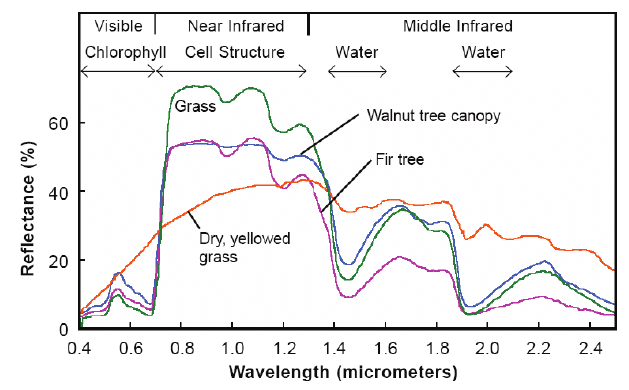
\includegraphics[width=0.5\textwidth]{img/Reflectance-spectra-of-different-types-of-green-vegetation-compared-to-a-spectral.png}
    \caption{Absorption spectrum of green vegetation \autocite[P. 5]{Smith2012}\label{fig:absorbtionVeg}}
\end{figure}
The \gls{NDVI} is an widely used index using the difference of the red and near infrared bands to determine the amount of green vegetation. 
\begin{equation}
    NDVI = \frac{Red-NIR}{Red+NIR}
    \label{equ:ndvi}
\end{equation}
For Landsat 8 and 9 data, channel 4 (red $640\ \text{nm} - 670\ \text{nm}$) and channel 5 (near infrared $850\ \text{nm} - 880\ \text{nm}$) where used.
As shown in \cref{fig:absorbtionVeg} healthy plants reflect near infrared and there is a sharp rise in reflectance between the two used channels at around $700\ \text{nm}$. 
%
This index is used for emissivity estimation for Land Surface Temperature calculation see \cref{equ:toa}, correlation with heat islands (since there is a negative correlation between those two values, due to the latent heat of evaporation reducing surface temperature at higher vegetation areas).
\begin{figure}[!htbp]
    \centering
    \begin{subfigure}{0.45\textwidth}
    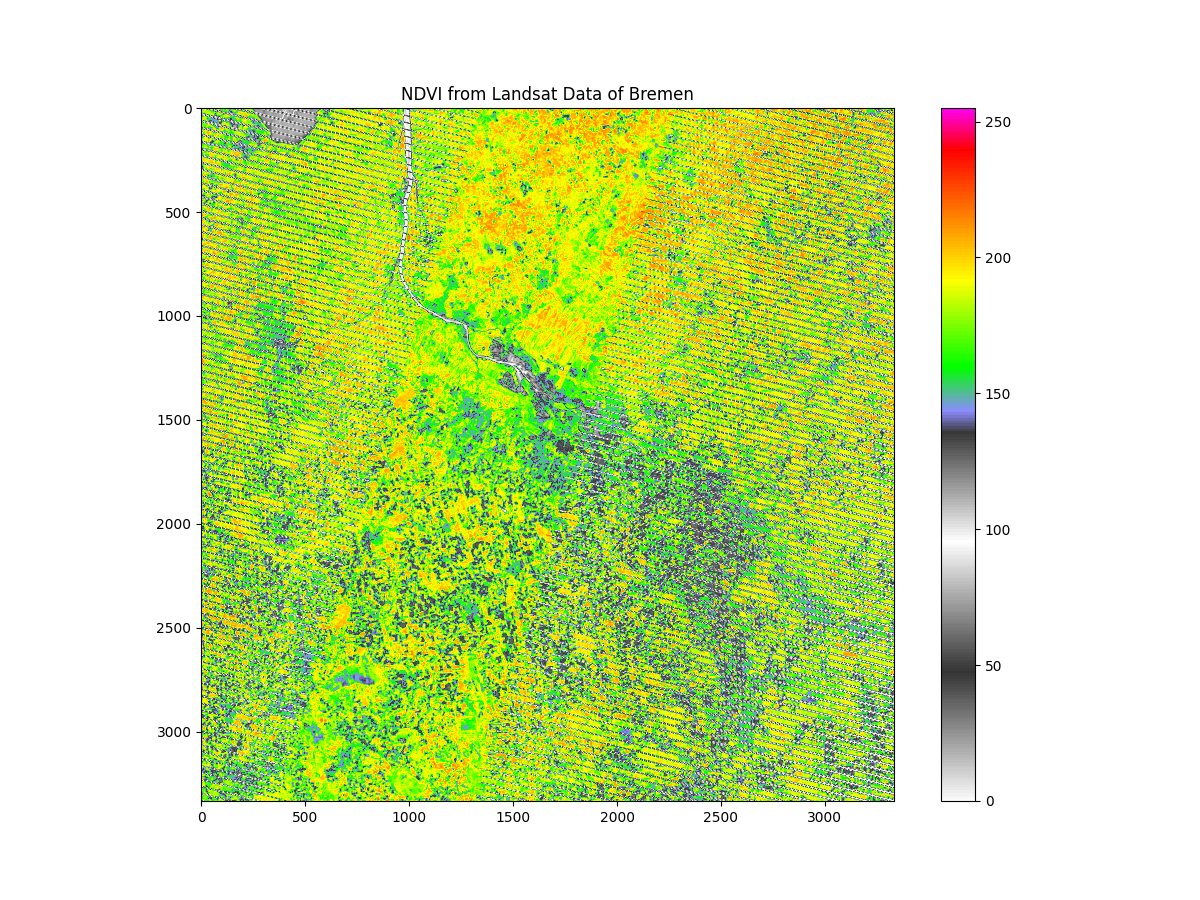
\includegraphics[width=\textwidth]{img/NDVI_LE07_L1TP_196023_20190723_20200825_02_T1__Bremen.png}
    \subcaption{NDVI of Bremen (Bands 5 and 6) using Landsat 7 data on 2019--07--23}
    \end{subfigure}
    \begin{subfigure}{0.45\textwidth}
    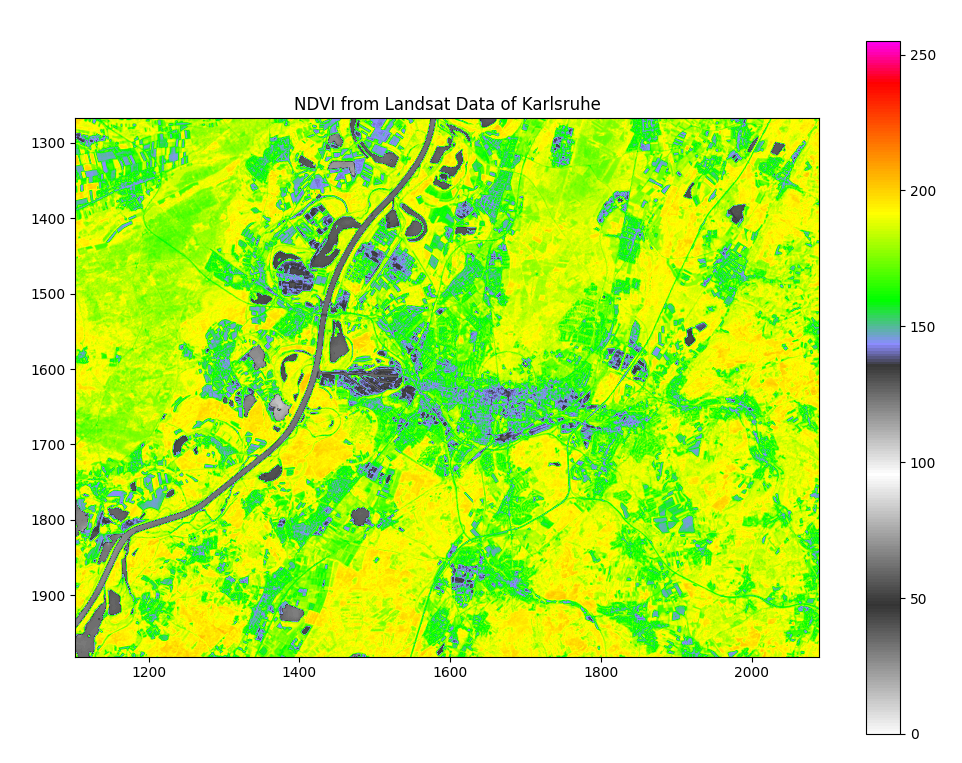
\includegraphics[width=\textwidth]{img/KarlsruheNDVI_Landsat8.png} 
    \subcaption{NDVI of Karlruhe (Bands 4 and 5) using Landsat 8 data on 2023--06--07}
    \end{subfigure}
    \caption{NDVI Images from the different satellites\label{fig:ndvi}}
\end{figure}
%\subsubsection{NDVI Colormap}\label{sec:colormap}
%When using a classical heat map with a color gradient from colder to warmer colors or a diverging color map (see \cref{fig:ndviPhoenixAzBad}), details of the image get lost and it is hard to distinguish plant heath, build up and vegetated areas and the difference between small \gls{NDVI} changes.
%To aid an intuitive understanding a specially created colormap can be used. 
%The color map was adapted for use in python from work of \texttt{public lab}\cite{ndviCmap} where it was developed in an attempt to create color-blind friendly \gls{NDVI} color maps.
%Values below 0.2 are areas with no vegetation.
%The color map used in \cref{fig:ndviPhoenixAz} uses a gradient of gray with a ``black-white-black
%white'' transition to allow higher dynamic range for non vegetation areas.
%For areas with an \gls{NDVI} $<$ 0.2 blue is used. Green values are low or unhealthy green vegetation or mixed use pixels. 
%Orange and red values correspond to thicker vegetation e.g.~forests, parks or green fields. 
%%
%Comparing \cref{fig:ndviPhoenixAz}  and \cref{fig:ndviPhoenixAzBad} where most of the desert surrounding the city has no green vegetation and the parts covered in vegetation can be clearly distinguished from the arid desert regions.
%Still the surface roughness can be seen quite well due to the gray scale gradient in the $<$ 0.2 \gls{NDVI} range.  
%%
%\begin{figure}[htbp]
% \centering
%    \begin{subfigure}{0.46\textwidth}
%    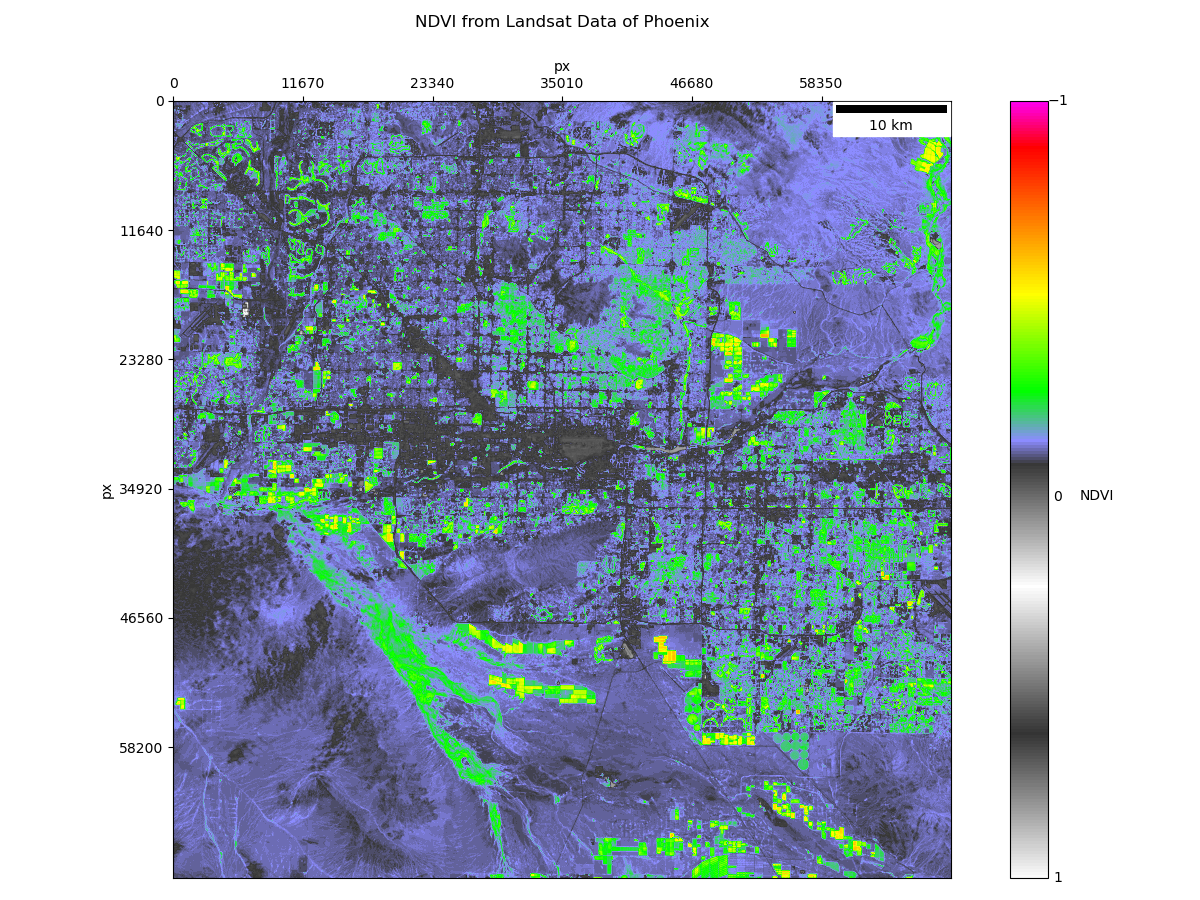
\includegraphics[width=\textwidth]{img/NDVI from Landsat Data of Phoenix.png} 
%    \subcaption{NDVI Image of Phoenix with the  VGYRM color map\label{fig:ndviPhoenixAz}}
%    \end{subfigure}
%    \begin{subfigure}{0.46\textwidth}
%    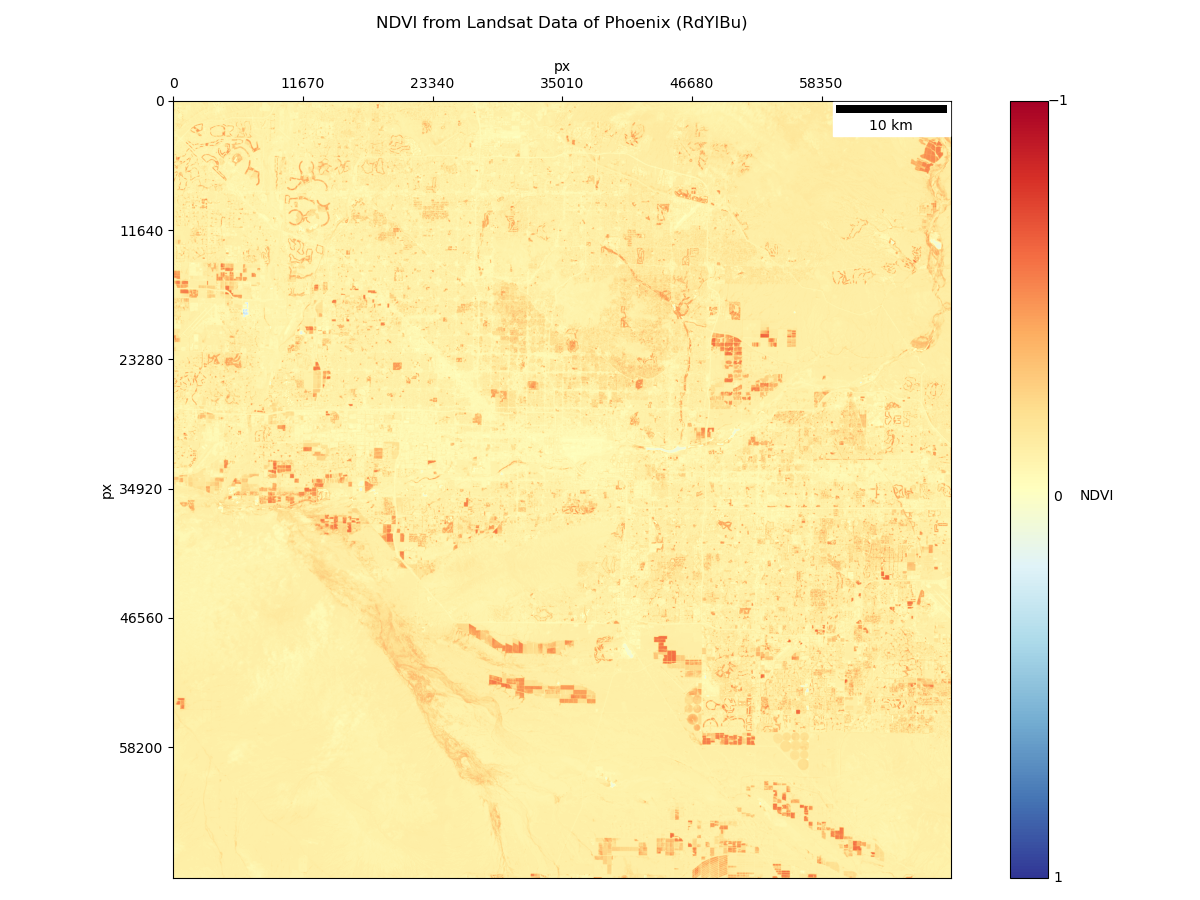
\includegraphics[width=\textwidth]{img/NDVI from Landsat Data of Phoenix (RdYlBu).png} 
%    \subcaption{NDVI Image of Phoenix with a RdYlBu gradient color map\label{fig:ndviPhoenixAzBad}}
%    \end{subfigure}
%    \caption{Different color maps used show the better ability to differentiate between green vegetation and desert and buildings within Phoenix\label{fig:ndvicomp}}
%\end{figure}

    \newpage
    \subsubsection{Heat Index}
    The \gls{HI}is a temperature index that takes sultriness into account and rates the impact of temperature and air humidity of the human body. 
    The output of this temperature scale (given in °C) is the apparent temperature, depending on relative air humidity. 
    The defined range is between 20 °C and 50°C dry bulb temperature and up to 90\% relative humidity~\cite[p. 862]{Steadman1979}. 
    The proposed heat index is based on a model human and takes wind chill and clothing into account, to produce a apparent temperature of human. 
    The heat index can be used as a good reference for non-extreme conditions. 
    Its biggest downside is the missing account for direct insolation on body temperature and comfort.
    The Heat Index later is used to compare different \glspl{UHI} with each other.
%%
    \subsection{Wet Bulb Globe Temperature}
    To account the impact of insolation on the human body and how it reacts to heat stress differently in different environmental condition s, the Wet Bulb Globe Temperature was developed. 
    Working under heat stress poses a serious health issue, for this the \gls{WBGT} was defined as EN ISO 7243:2017, calculating the thermal load on the human body\cite{Iso7243_2017}
    Heat exchange between the human body and the environment is dominated by evaporation of secreted sweat.
    The efficiency of this process is determined by the vapor pressure, that is influenced by temperature difference and the humidity difference. %TODO ref paper with caves
    The Heat Index is a simple way of calculating this efficiency that does not take radiant heat into account, the WBGT does incorporated this effect as well as clothing in this process. 
    \subsection{Urban Air Quality}
    Large urbanized areas are susceptible to air pollution due to increased combustion and industrial activity. % TODO Numerous studies \cite{Kanakidou2011}
    One major pollutant with a significant health impact is tropospheric ozone that is produced in larger quantities within higher temperature environments (see~\cite{Ebi2008}). 
    Ozone is mainly produced when (anthropogenic) NO\textsubscript{x} emissions and other \glspl{VOC} react with volatile organic compounds. %todo source
    The creation of ozone is dependent on temperature, increasing between 2.2 and 3.2 ppbv/°C depending on NO\textsubscript{x}
    %\subsection{Models and Theories}
\newpage
\section{Image Processing}\label{sec:imgProcessing}
    Using remote sensing data for scientific purposes requires a 
    \begin{itemize} 
      \item[a] systematic
      \item[b] reproducible
      \item[c] verifiable 
    \end{itemize}%
    way of detecting patterns and information within the data. \\
    The field of image processing and machine learning has developed a wide range of tools that are used in many different fields over the past decades. % TODO might want to add examples here ?

    \subsection{Machine Learning}\label{sec:ml}
    The term machine learning describes a set of algorithms that use a set of training data, detect statistical correlations using different weights to approximate this data. %TODO external source 
    These approximations can be stored and be used to detect the same features within new but similar data.
    Different machine learning techniques are used for for different use cases and areas.
    %In total 
%
  In the next sections the image processing steps are described from a technical perspective and the underlying mathematical frameworks are discussed.
%
    \subsection{Data Processing Pipeline}
    An image or data processing pipeline is a chained list of processing steps, that allows to feed different data through the same algorithm. 
    Many different data processing and machine learning \glspl{lib} use these to allow flexibility and modularity of the steps in data processing (e.g.\ the used~\cite{scikit-learn},~\cite{keras} or~\cite{gluon}). 
    The data processing was used using scikit-learn pipeline for data analysis as well as multiple other \glspl{lib}. 
    In \cref{fig:pipeline} the overview of the different steps within the data processing can be seen.
%
    \begin{figure}[!htbp]
       \begin{subfigure}[b]{0.50\textwidth}
         \begin{tikzpicture}[node distance=2cm, auto, scale=.5, on grid]
  \node (start) [startstop, text width=0.7\textwidth] {Start};
  \node (input) [io, below of=start, text width=0.6\textwidth]{Landsat 8\ \& 9 Image};
  \node (cut) [process, below of=input, text width=0.9\textwidth]{Cut to AOI};
  \node (features) [process, below of=cut, text width=0.9\textwidth]{Gabor Feature Extraction};
  \node (kmeans) [process, below of=features, text width=0.9\textwidth]{KMeans clustering};
  \node (stat1) [process, below of=kmeans, text width=0.9\textwidth]{Statistical analysis of different classes};
  \node (stat2) [process, below of=stat1, text width=0.9\textwidth]{manual class name assignment};
  \node (verif) [process, below of=stat2, text width=0.9\textwidth]{verification of classification};
  \node (diff) [process, below of=verif, text width=0.9\textwidth]{diff analysis of LU/LC classes};
  \node (stop) [startstop, below of=diff,text width=0.7\textwidth] {Stop};

  \draw[arrow] (start) -- (input);
  \draw[arrow] (input) -- (cut);
  \draw[arrow] (cut) -- (features);
  \draw[arrow] (features) -- (kmeans);
  \draw[arrow] (kmeans) -- (stat1);%(randomforest);
  %\draw[arrow] (randomforest) -- (stat1);
  \draw[arrow] (stat1) -- (stat2);
  \draw[arrow] (stat2) -- (verif);
  \draw[arrow] (verif) -- (diff);
  \draw[arrow] (diff) -- (stop);
\end{tikzpicture}

         \caption{Processing pipeline for developing the model}\label{fig:pipelineTraining}
       \end{subfigure}
       \begin{subfigure}[b]{0.50\textwidth}
         \begin{tikzpicture}[node distance=2cm, auto, scale=.5, on grid]
  \node (start) [startstop, text width =0.7\textwidth] {Start};
  \node (input) [io, below of=start, text width =0.6\textwidth]{Landsat 7\& 8 Image};
  \node (cut) [process, below of=input, text width = 0.9\textwidth]{Cut to AOI};
  \node (features) [process, below of=cut, text width = 0.9\textwidth]{Gabor Feature Extraction};
  \node (randomforest) [process, below of=features, text width = 0.9\textwidth]{Surface Classification \\using the trained model};
  \node (stat1) [process, below of=randomforest, text width = 0.9\textwidth]{Urban area detection using Random Forrest};
  \node (stat2) [process, below of=stat1, text width = 0.9\textwidth]{Statistical analysis of image areas};
  \node (diff) [process, below of=stat2, text width = 0.9\textwidth]{LU/LC change detection};
  \node (uhi) [process, below of=diff, text width = 0.9\textwidth]{UHI detection};
  \node (timeline) [process, below of=uhi, text width = 0.9\textwidth]{analyse change over time};

  \draw[arrow] (start) -- (input);
  \draw[arrow] (input) -- (cut);
  \draw[arrow] (cut) -- (features);
  \draw[arrow] (features) -- (randomforest);
  \draw[arrow] (randomforest) -- (stat1);
  \draw[arrow] (stat1) -- (stat2);
  \draw[arrow] (stat2) -- (diff);
  \draw[arrow] (diff) -- (uhi);
  \draw[arrow] (uhi) -- (timeline);
\end{tikzpicture}

         \caption{Data Processing pipeline with the trained Model}\label{fig:pipelineTrained}
       \end{subfigure}
       \caption{The image processing overview\label{fig:pipeline}}
     \end{figure}
%
\newpage
\subsection{Gabor Feature Detection}\label{sec:gabor}

The Gabor filter is an linear filter, that uses a convolution of an image with a wavelet created by rotating a sine modulated Gaussian, this kernel type is also called the \textit{gabor wavelet}. 
In image processing this algorithm is used as an feature extraction algorithm to extract and analyse texture and structures with different sizes within the image~(\cite{Cerdan1993}). 
By rotating the kernel and changing the frequency, different textures are extracted from the image.
%
Mathematically the Gabor-filter is defined by
    \begin{equation}
      g(x,y; \lambda, \theta, \phi, \sigma, \gamma) = \exp \left(- \frac{x'^2 + \gamma^2\cdot y'^2}{2\sigma^2}\right) \cdot \exp \left[i \left(2\pi\frac{x}{\lambda} + \phi \right)\right] 
    \end{equation}
    With $ x' = x \cos(\phi) + y \sin(\phi)~\text{and}~y' = -x \sin(\phi) + y \cos(\phi)$.
%
    The x and y parameter determine the kernel size, this parameter should be chosen based on the image size and expected structure length.\\
    $\gamma$ is the aspect ratio of the kernel, with $\gamma = 1$ the kernel is round, for smaller $\gamma$ the kernel becomes a more eccentric ellipse.\\
    $\phi$ is the angle of rotation of the sine component of the kernel. \\
    $\theta$ is the angle of rotation of the kernel, detecting differently oriented features.\\
    $\lambda$ is the wavelength of the sine wave. \\
    $\sigma$ is the standard deviation of the Gaussian distribution\\ \\
%
%    
    %TODO add more accurate description of parameters
%
    To detect different structures of different scales within the image, a filter bank can be created by combining multiple filters and varying $\phi$, $\sigma$ and $\theta$.\\
%
    After the convolution of the image with the filter bank, the resulting set of detected features can be used as an input into different algorithms.
    \Cref{fig:gaborExample} shows different kernel sizes and rotations on an satellite image of Bremen. 
    It can be seen that the different structures such as fields (seen in \cref{fig:feat02} and \cref{fig:feat05}) or larger structures and water bodies (seen in \cref{fig:feat01} and \cref{fig:feat03}).
    The output of the filter is an tensor that contains a binary image sized matrix per filter. Each layer provides meta information for each pixel, if it is part of a larger scale texture or pattern. 
    This meta information is used to add additional features for the surface classification (\cref{sec:classification}) using K-Means (in training) and to allow better classification using the random forest model.
%
    \begin{figure}[!htbp]
       \centering
     \begin{subfigure}[b]{0.45\textwidth}
         \centering
         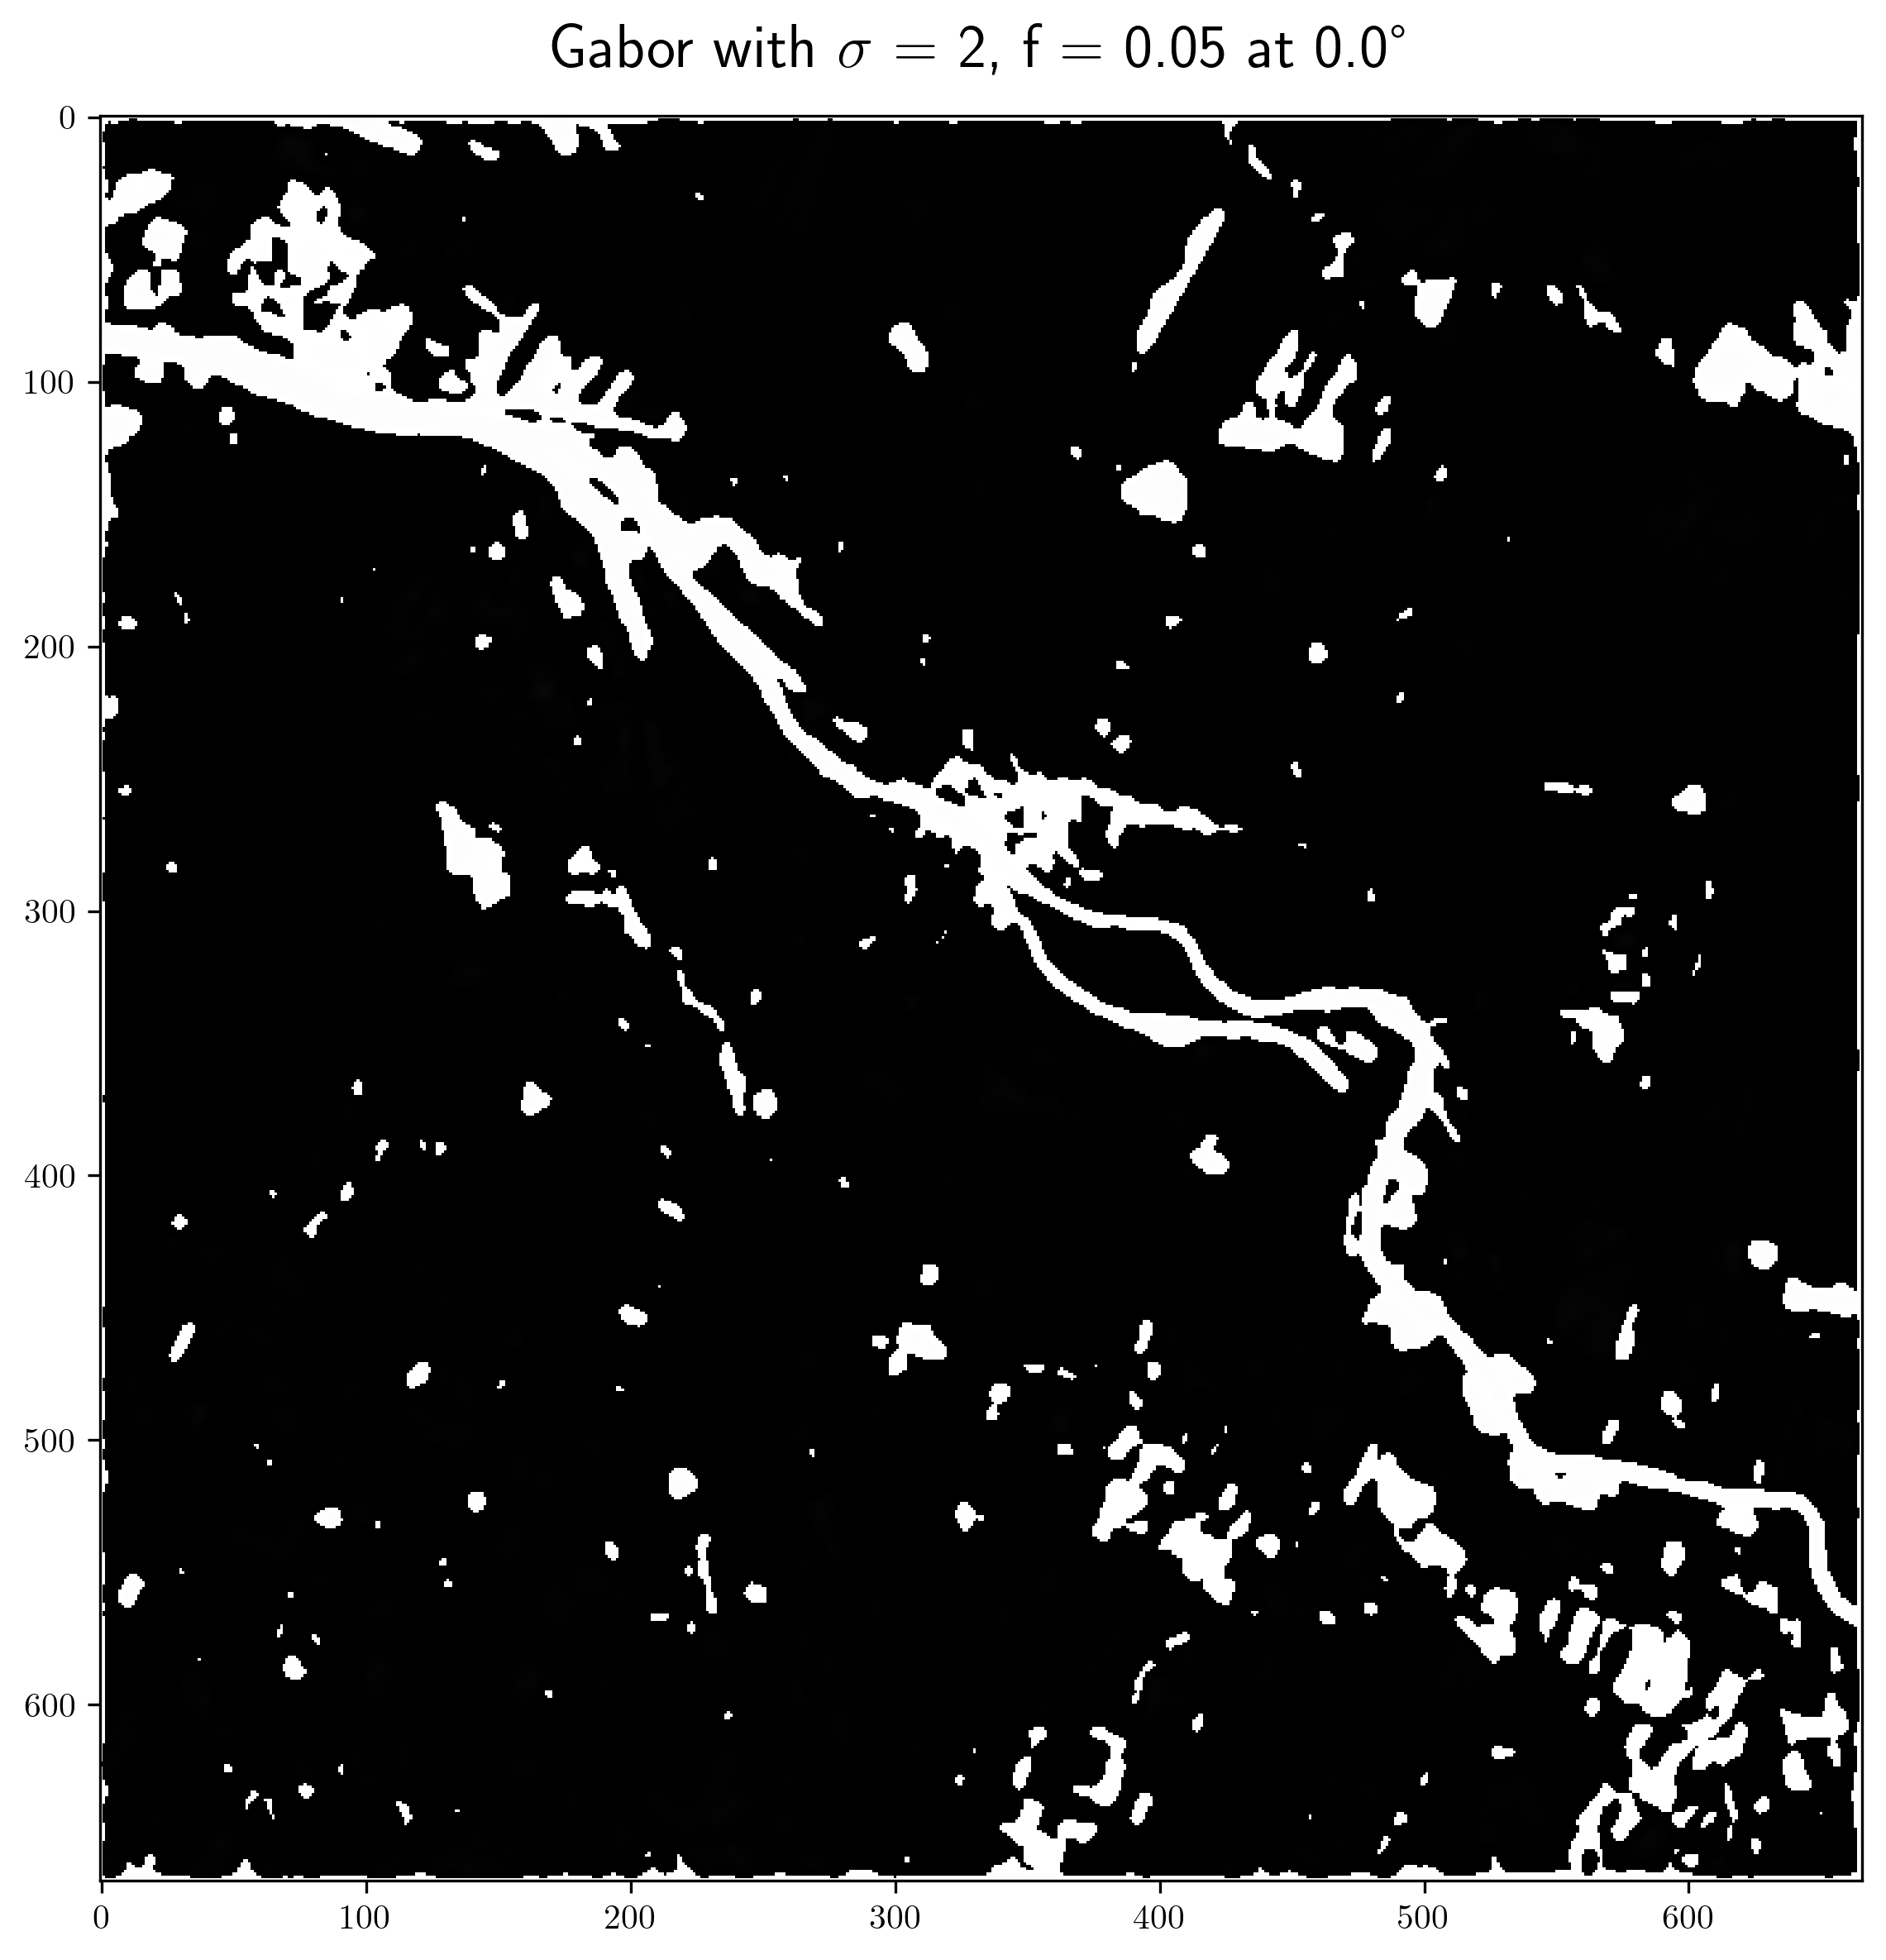
\includegraphics[width=\textwidth]{img/Features_2_005_0.png}
         \caption{Kernel with $\sigma$ = 2, f = 0.05 and 0 ° rotation}\label{fig:feat01}
     \end{subfigure}
     \hfill
     \begin{subfigure}[b]{0.45\textwidth}
         \centering
         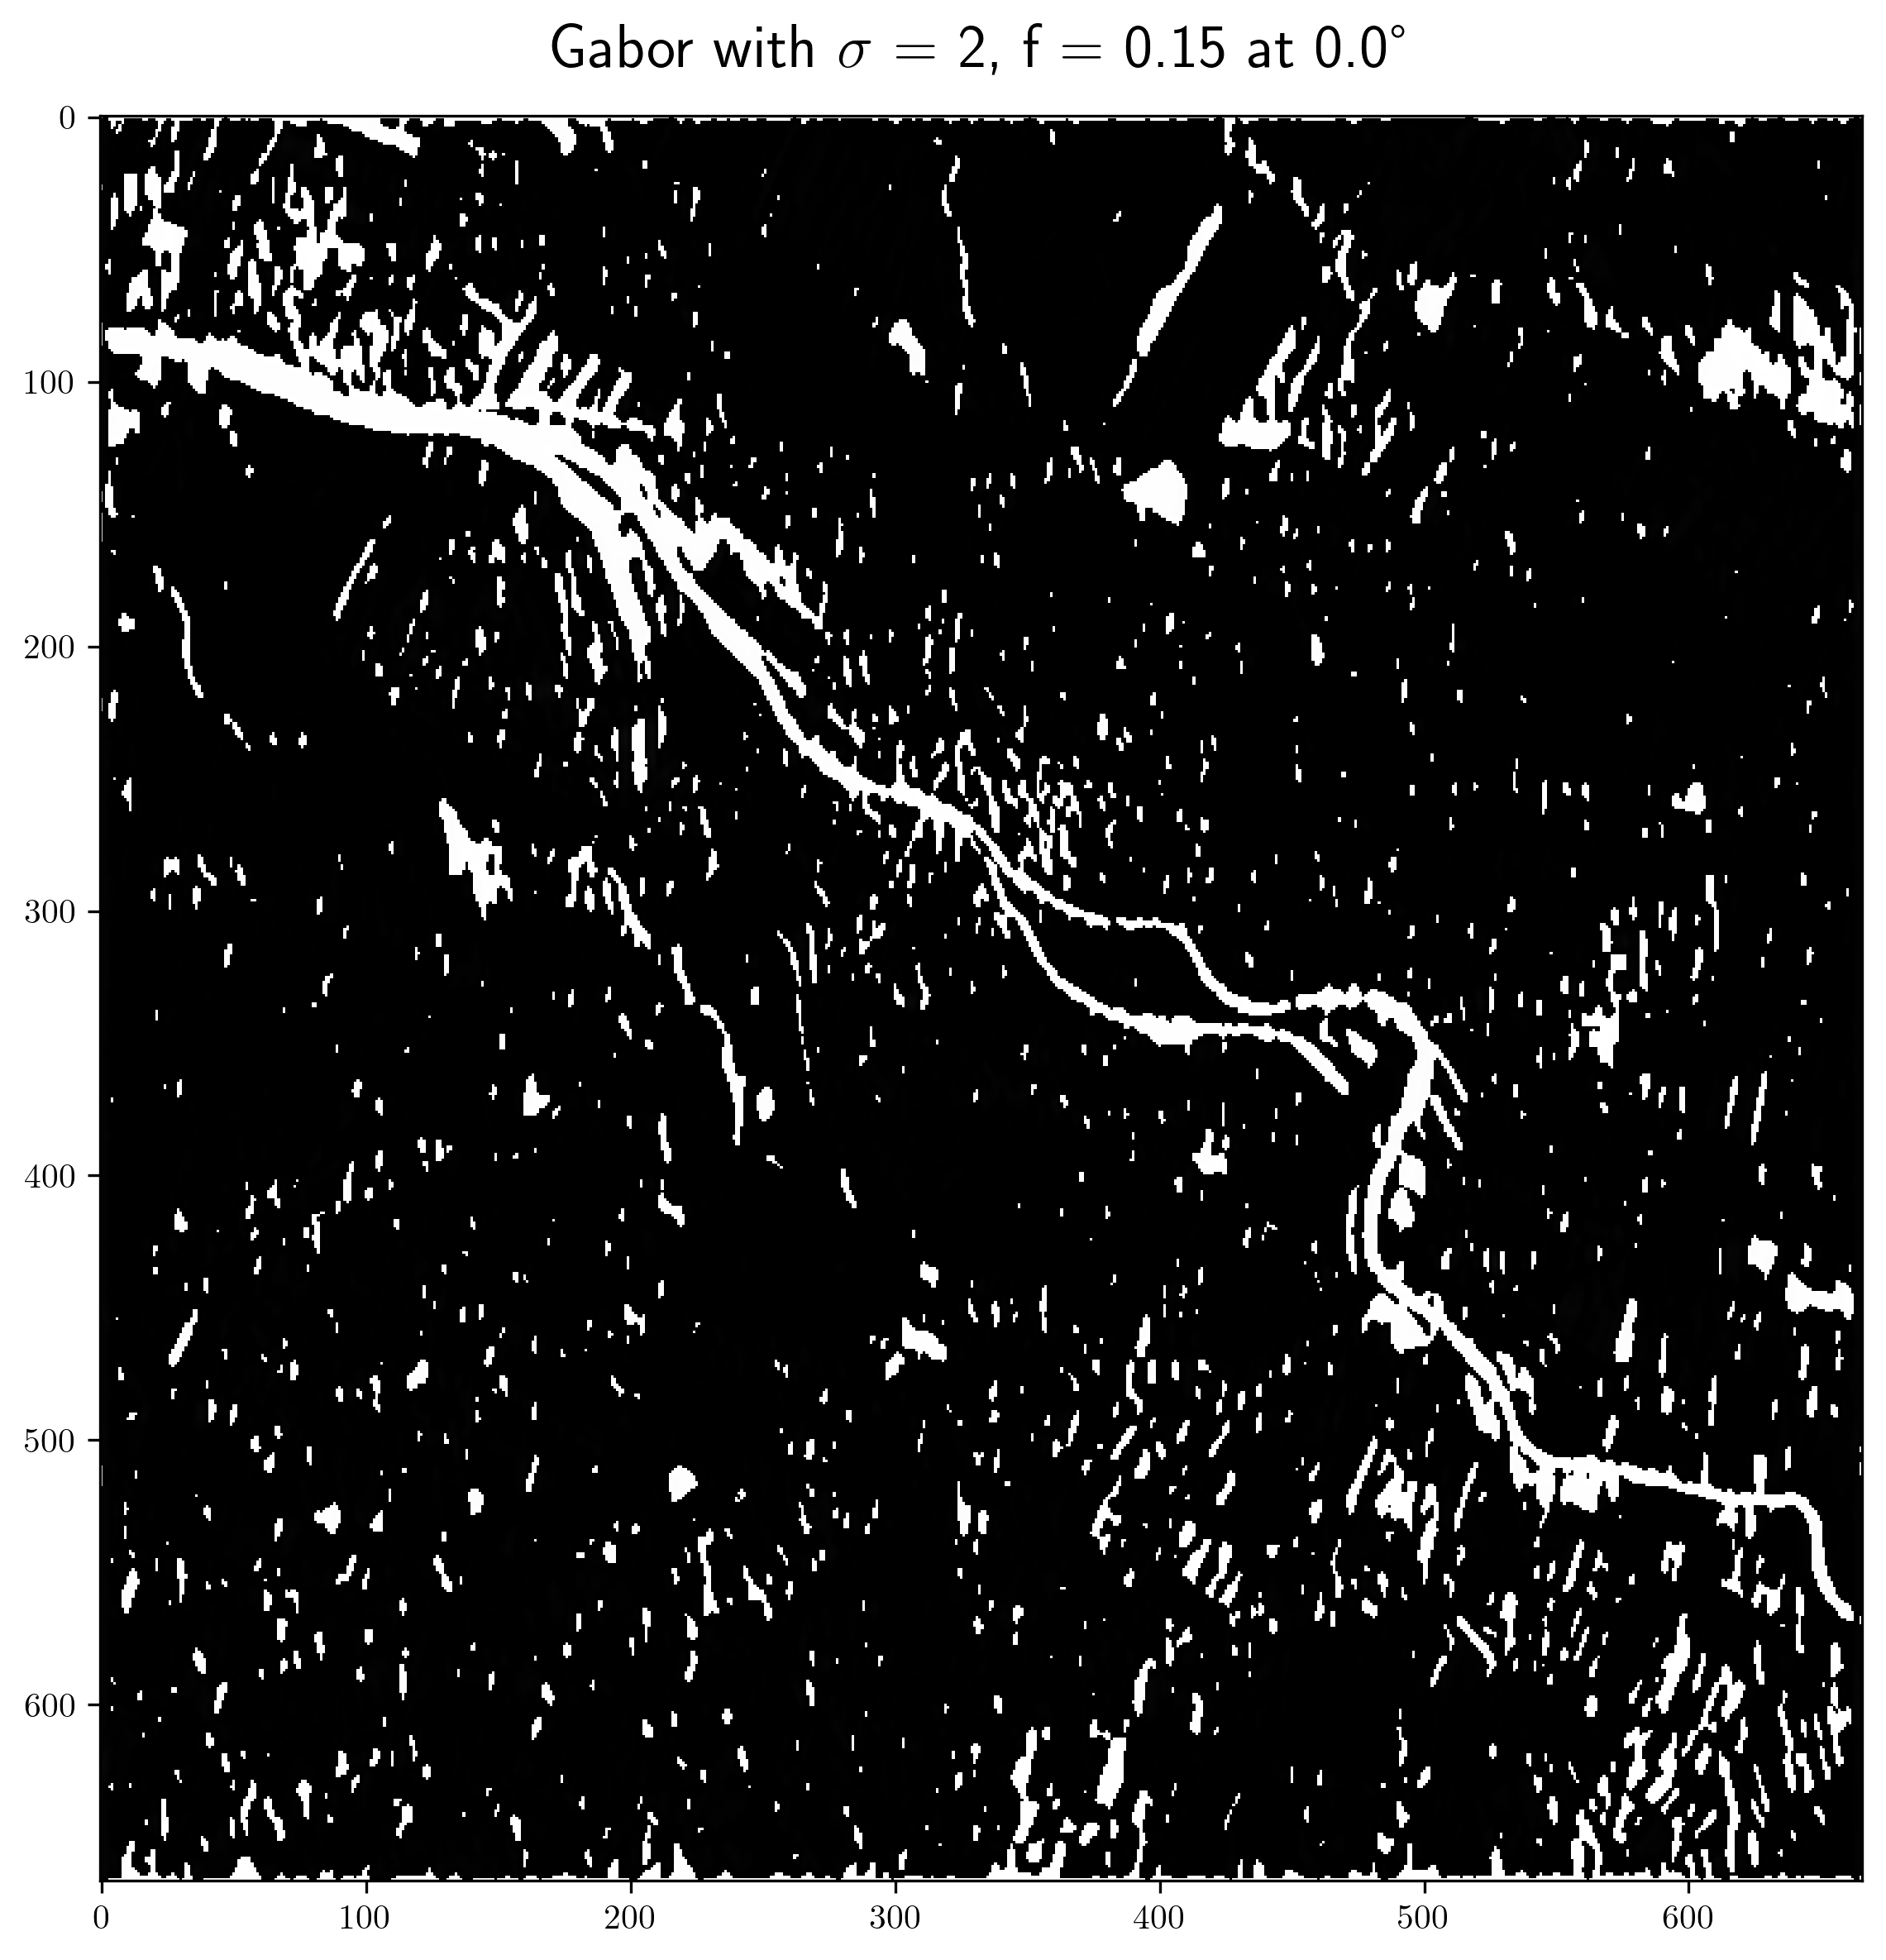
\includegraphics[width=\textwidth]{img/Features_2_015_0.png}
         \caption{Kernel with $\sigma$ = 2, f = 0.15 and 0 ° rotation}\label{fig:feat02}
     \end{subfigure}

     \begin{subfigure}[b]{0.45\textwidth}
         \centering
         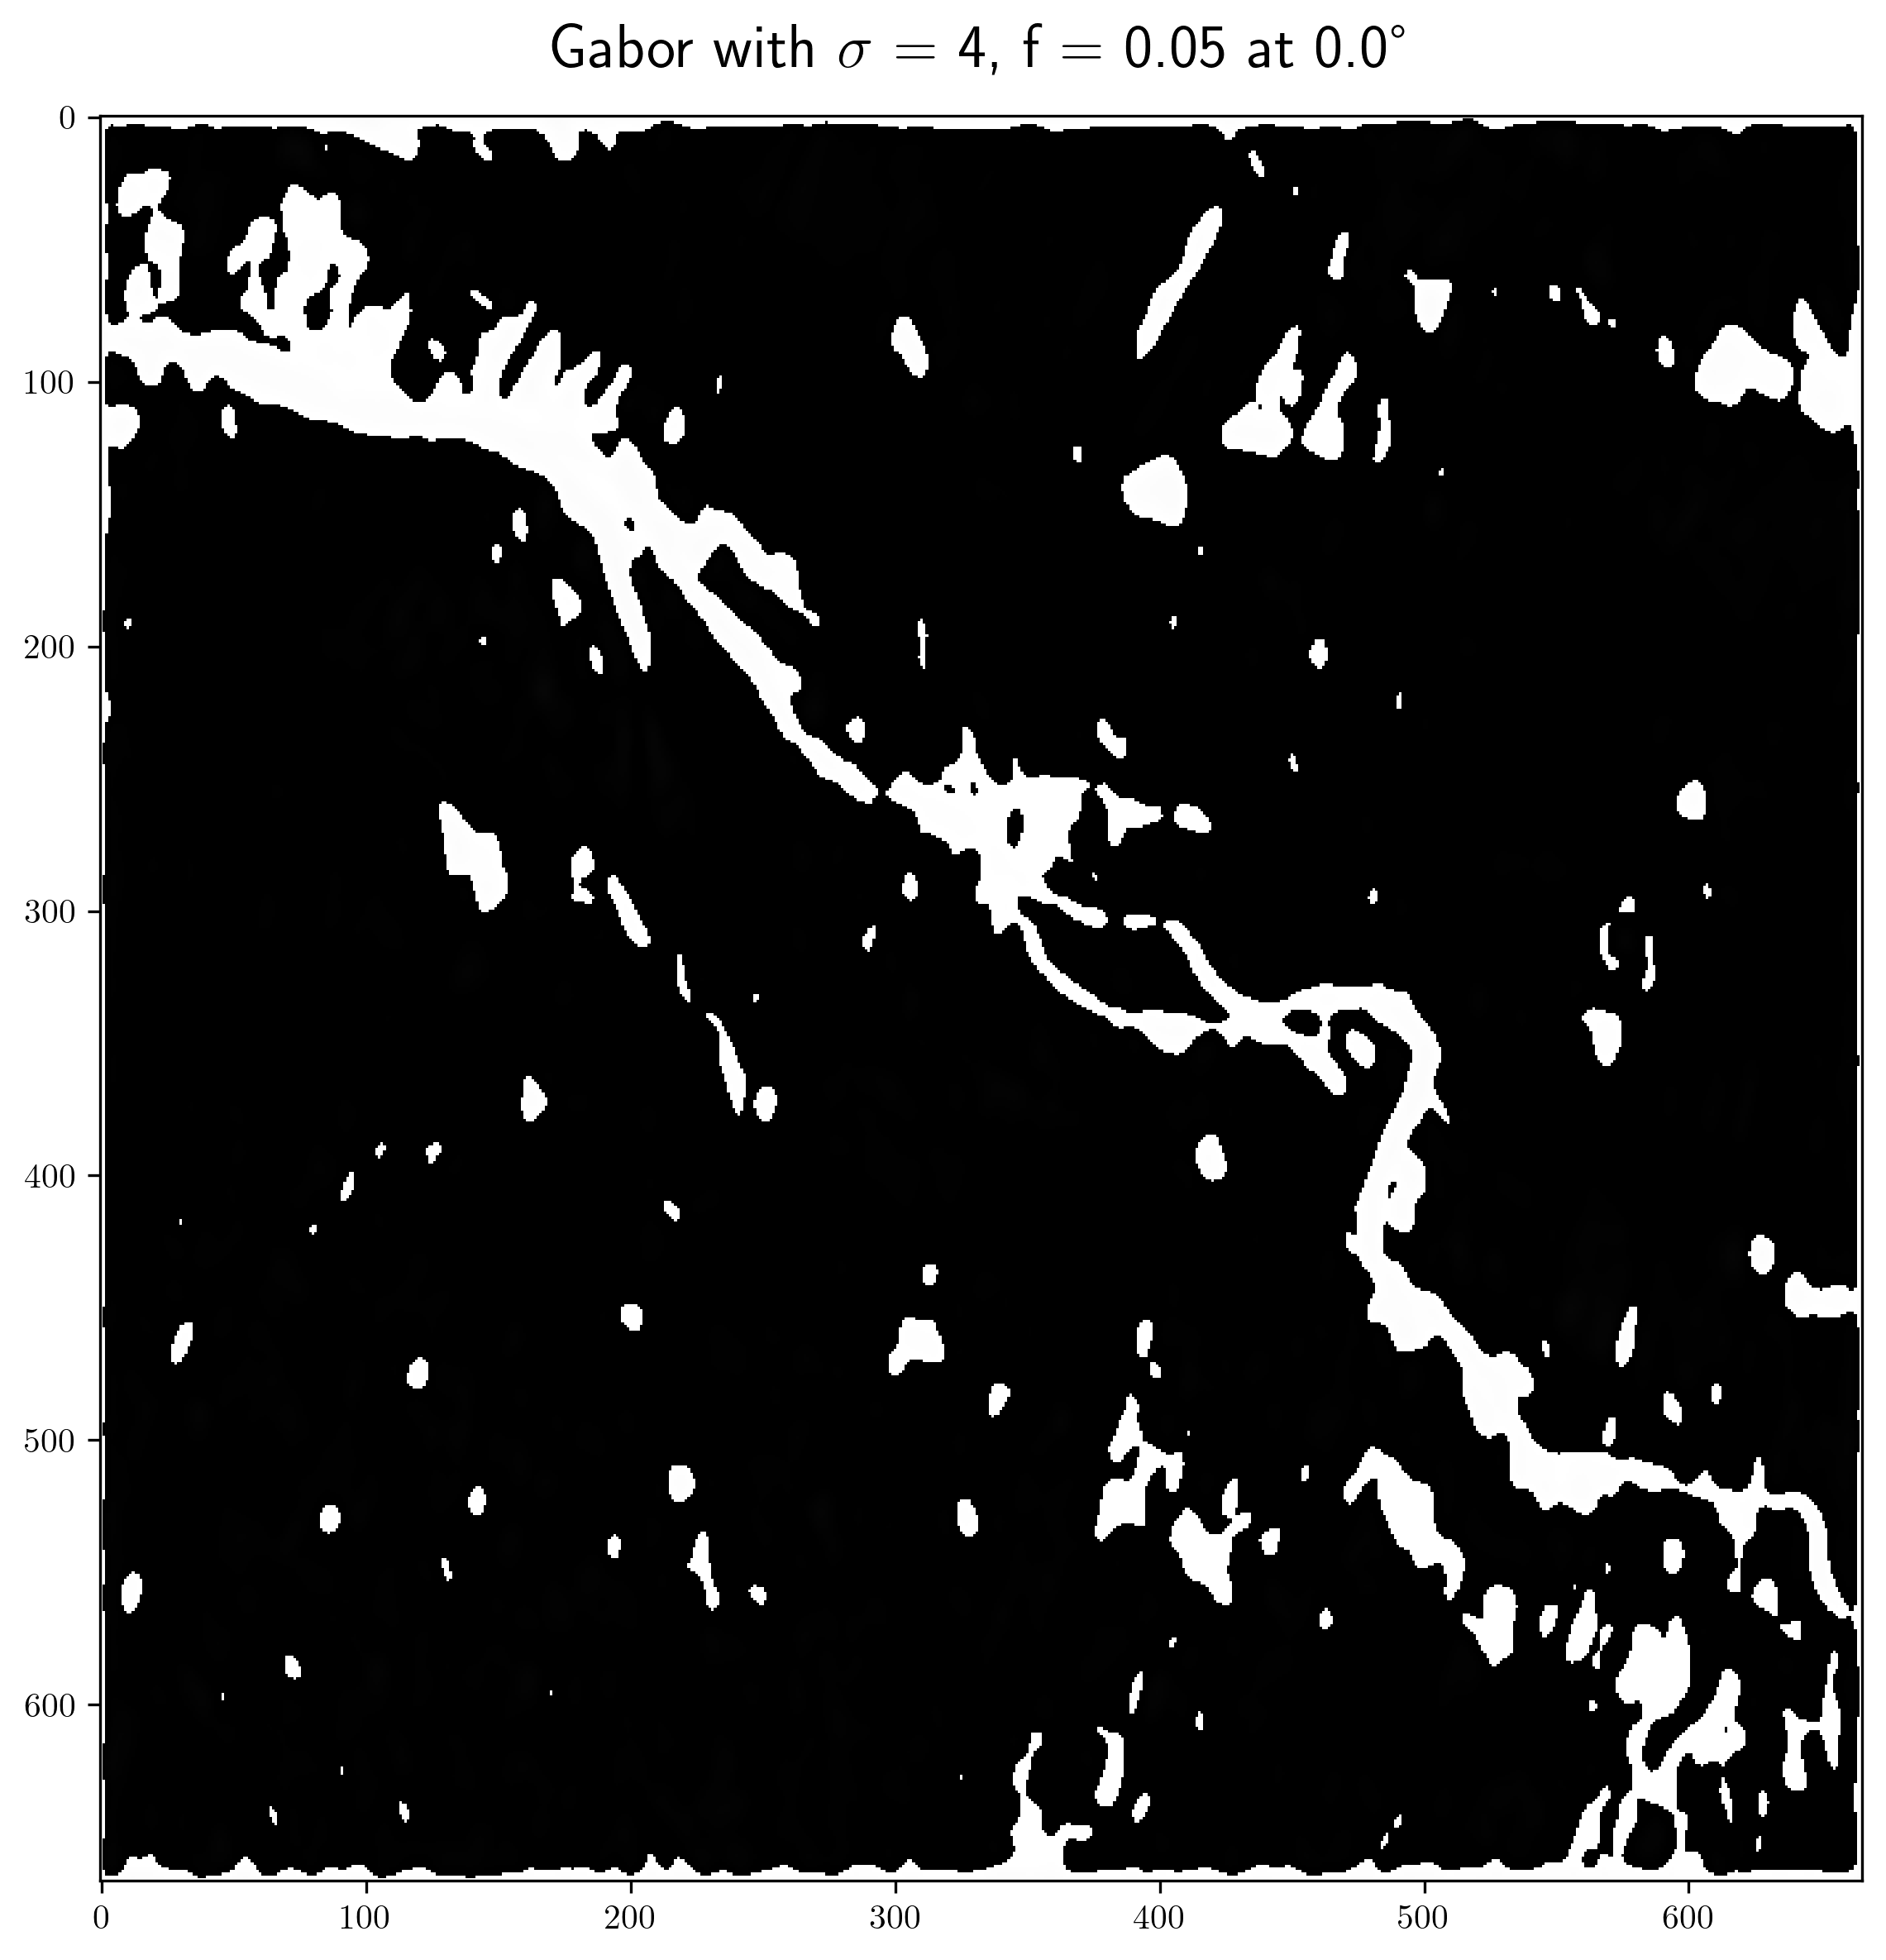
\includegraphics[width=\textwidth]{img/Features_4_005_0.png}
         \caption{Kernel with $\sigma$ = 4, f = 0.05 and 0 ° rotation}\label{fig:feat03}
     \end{subfigure}
     \hfill
     \begin{subfigure}[b]{0.45\textwidth}
         \centering
         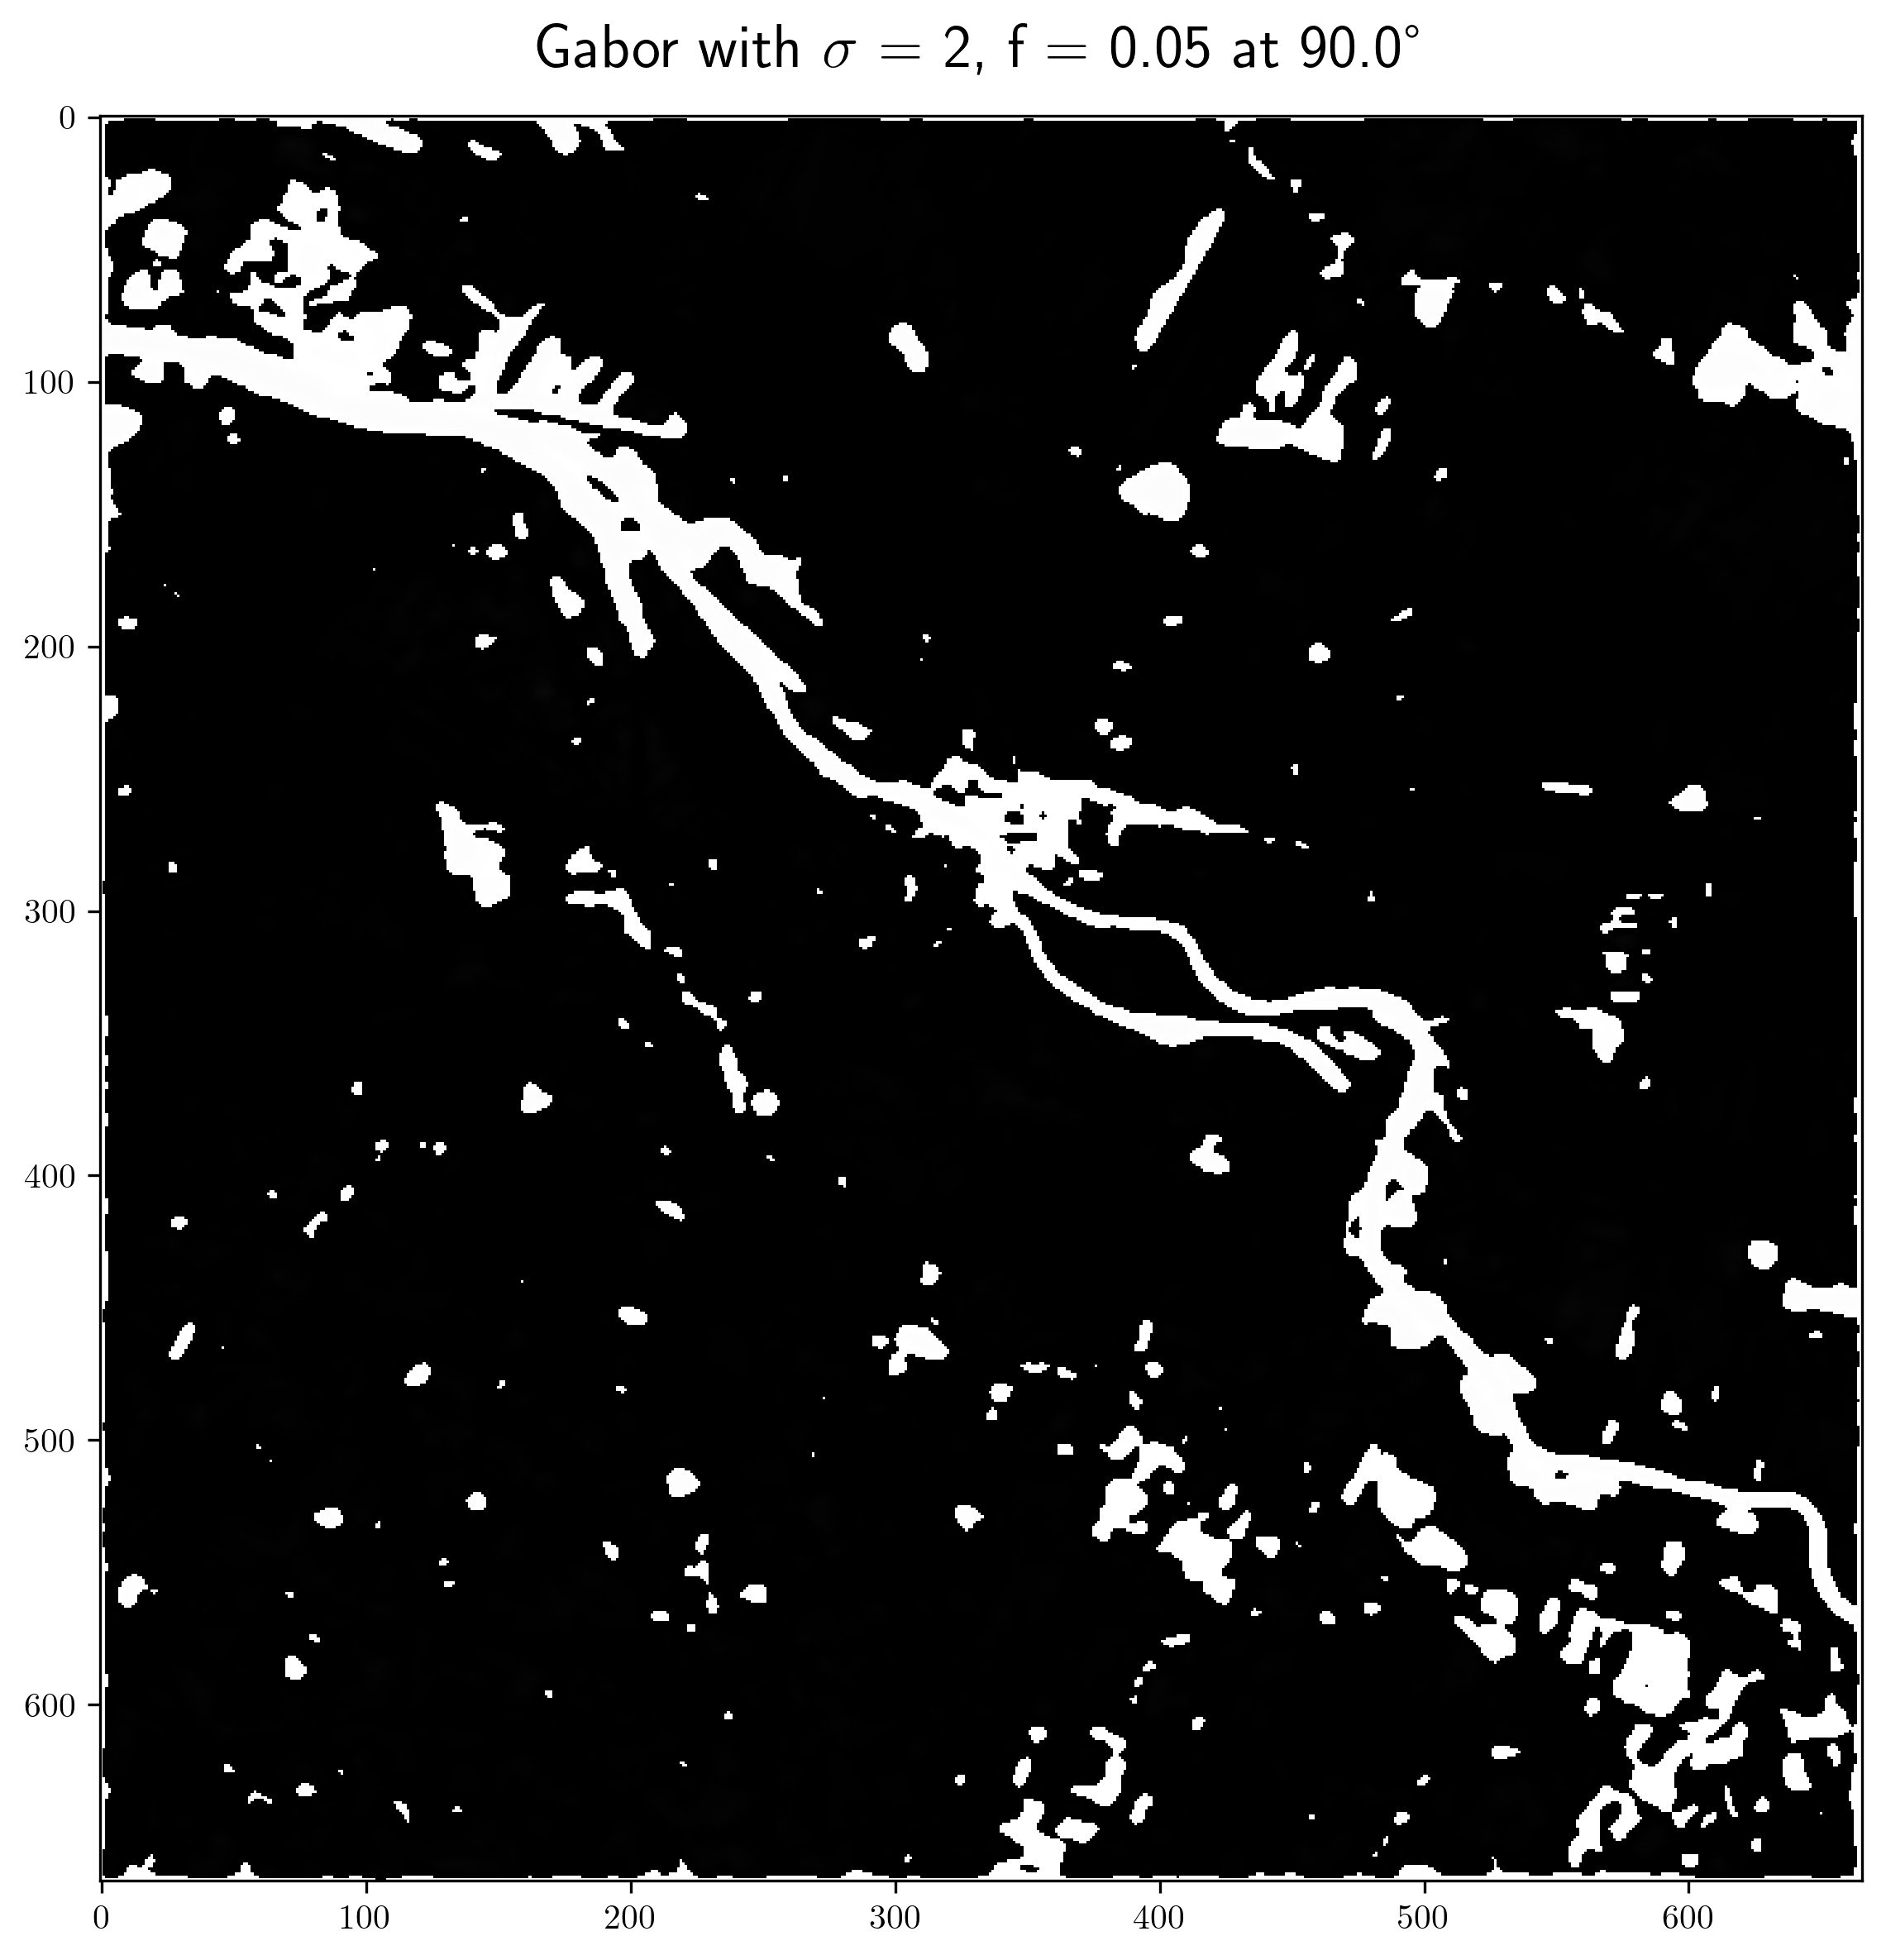
\includegraphics[width=\textwidth]{img/Features_2_005_90.png}
         \caption{Kernel with $\sigma$ = 2, f = 0.05 and 90 ° rotation}\label{fig:feat04}
     \end{subfigure}

     \begin{subfigure}[b]{0.45\textwidth}
         \centering
         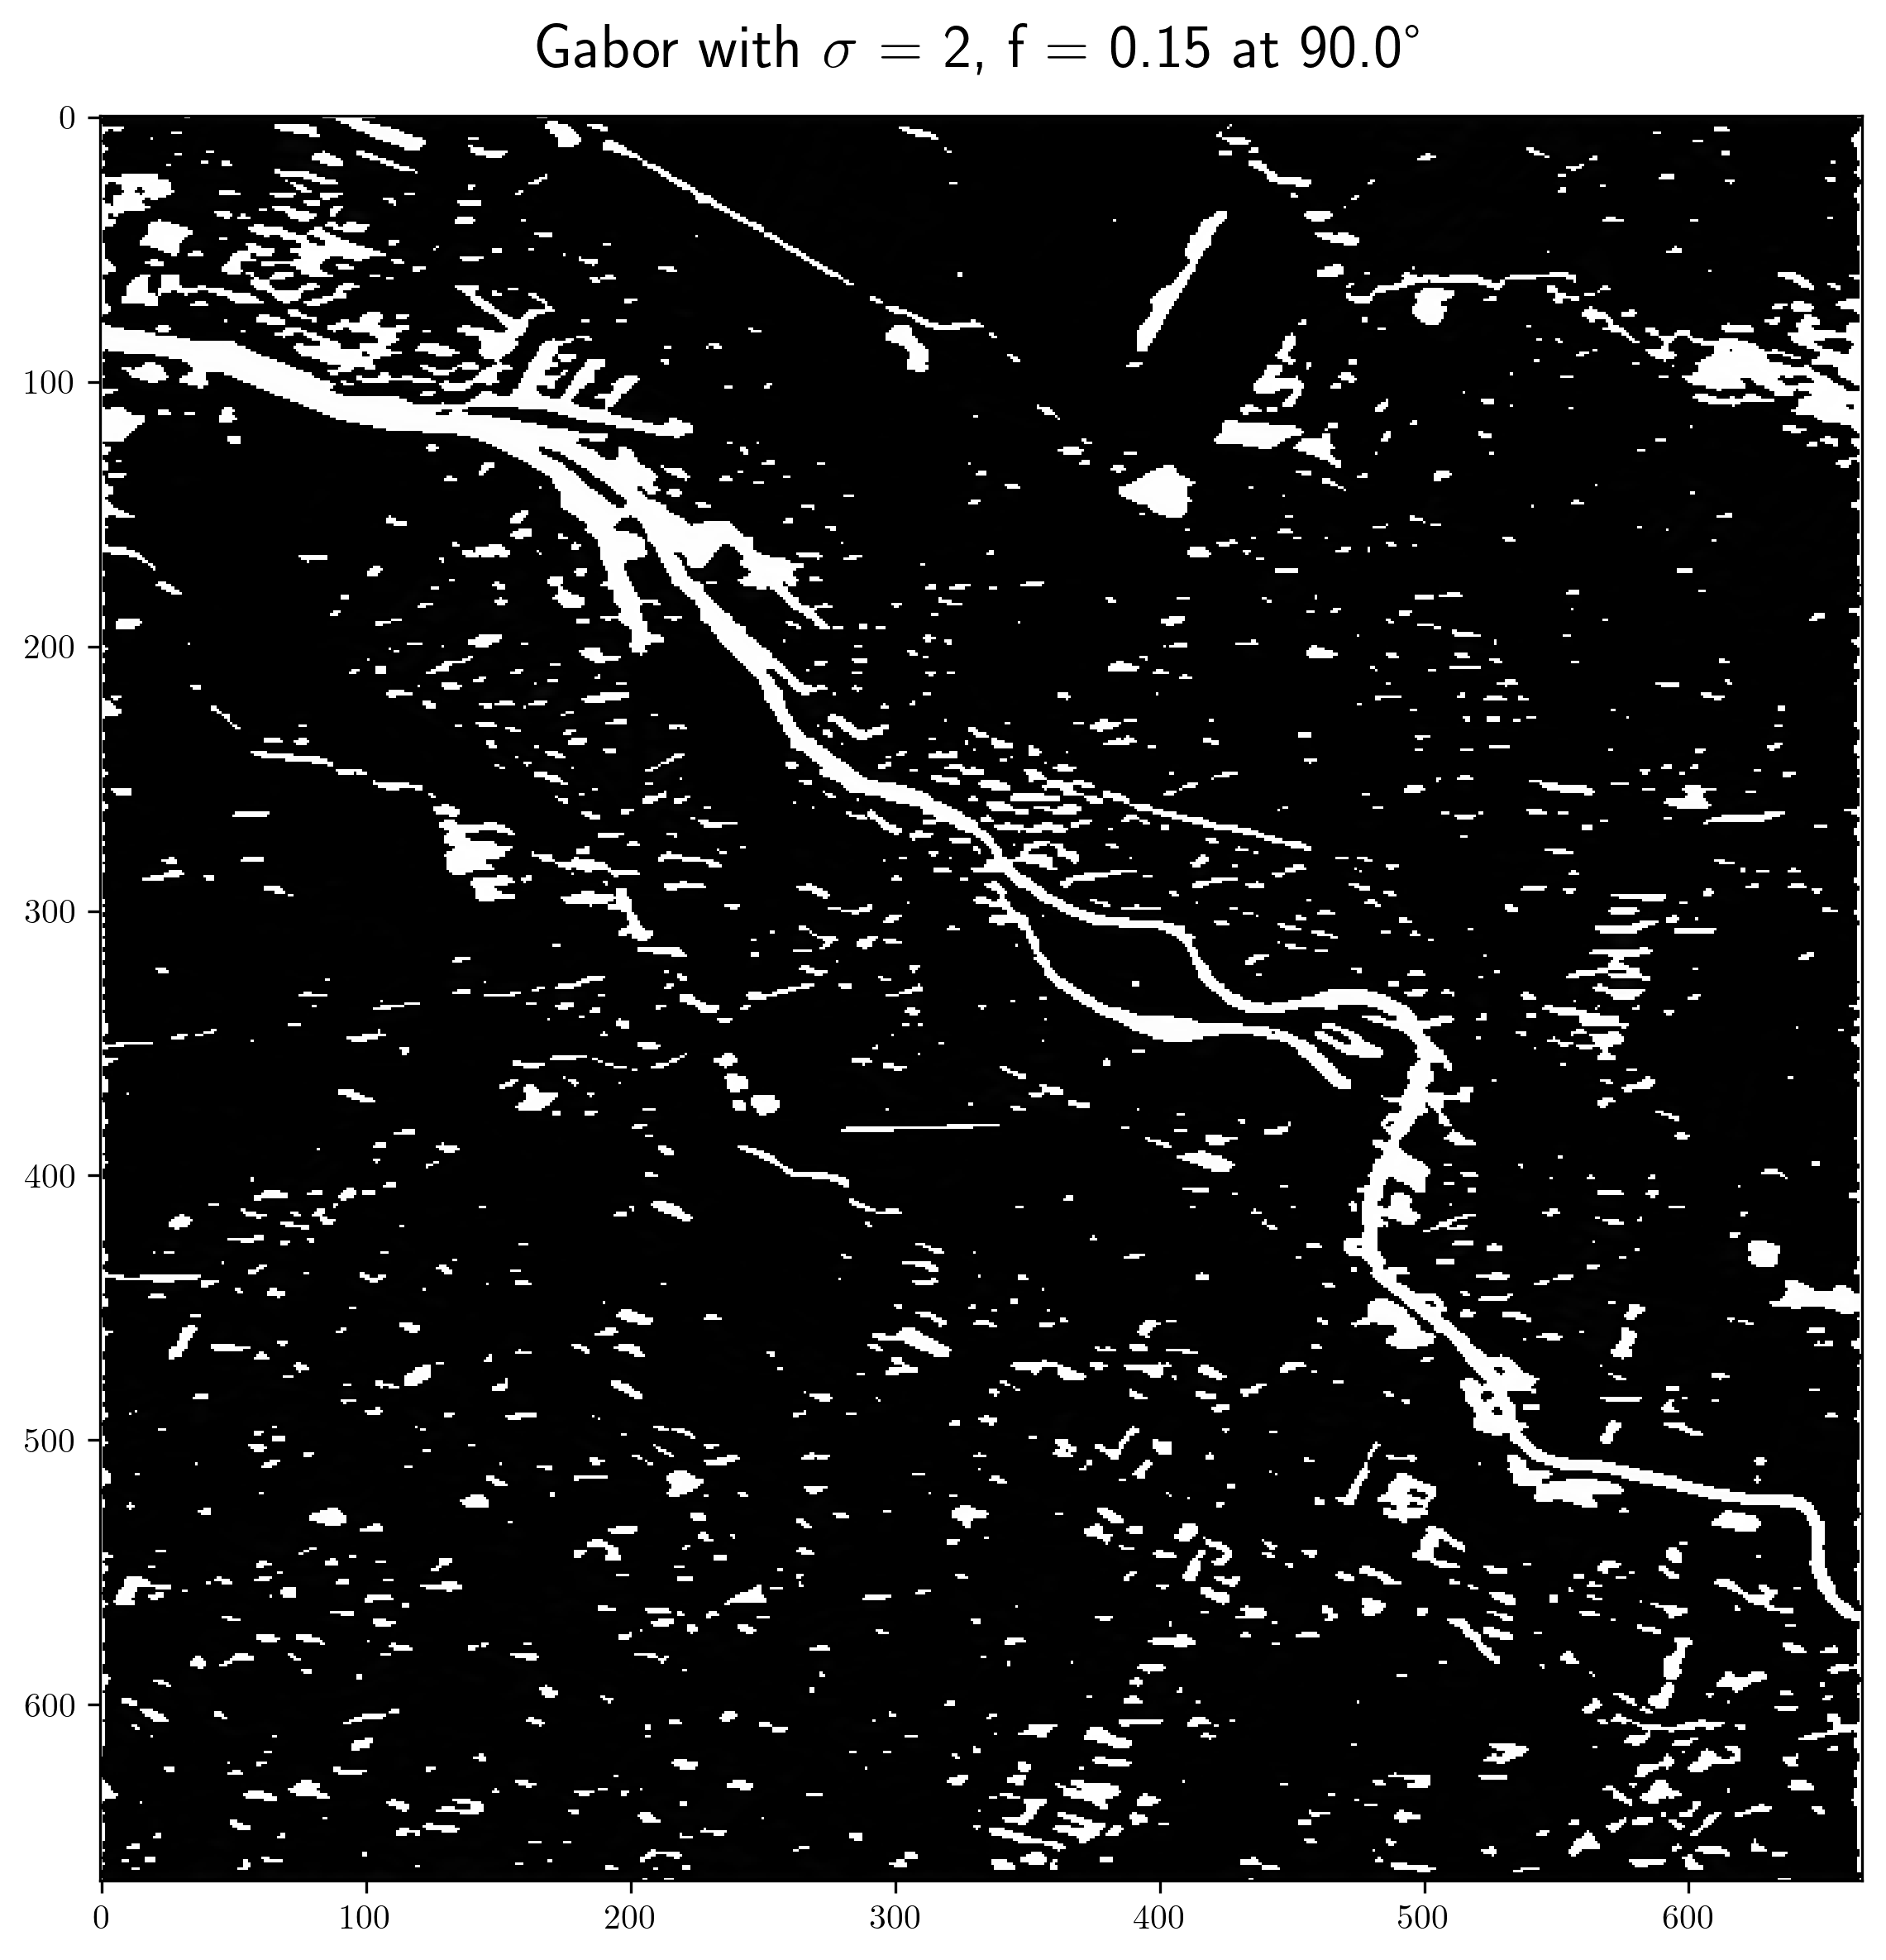
\includegraphics[width=\textwidth]{img/Features_2_015_90.png}
         \caption{Kernel with $\sigma$ = 2, f = 0.15 and 90 ° rotation}\label{fig:feat05}
     \end{subfigure}
     \hfill
     \begin{subfigure}[b]{0.45\textwidth}
         \centering
         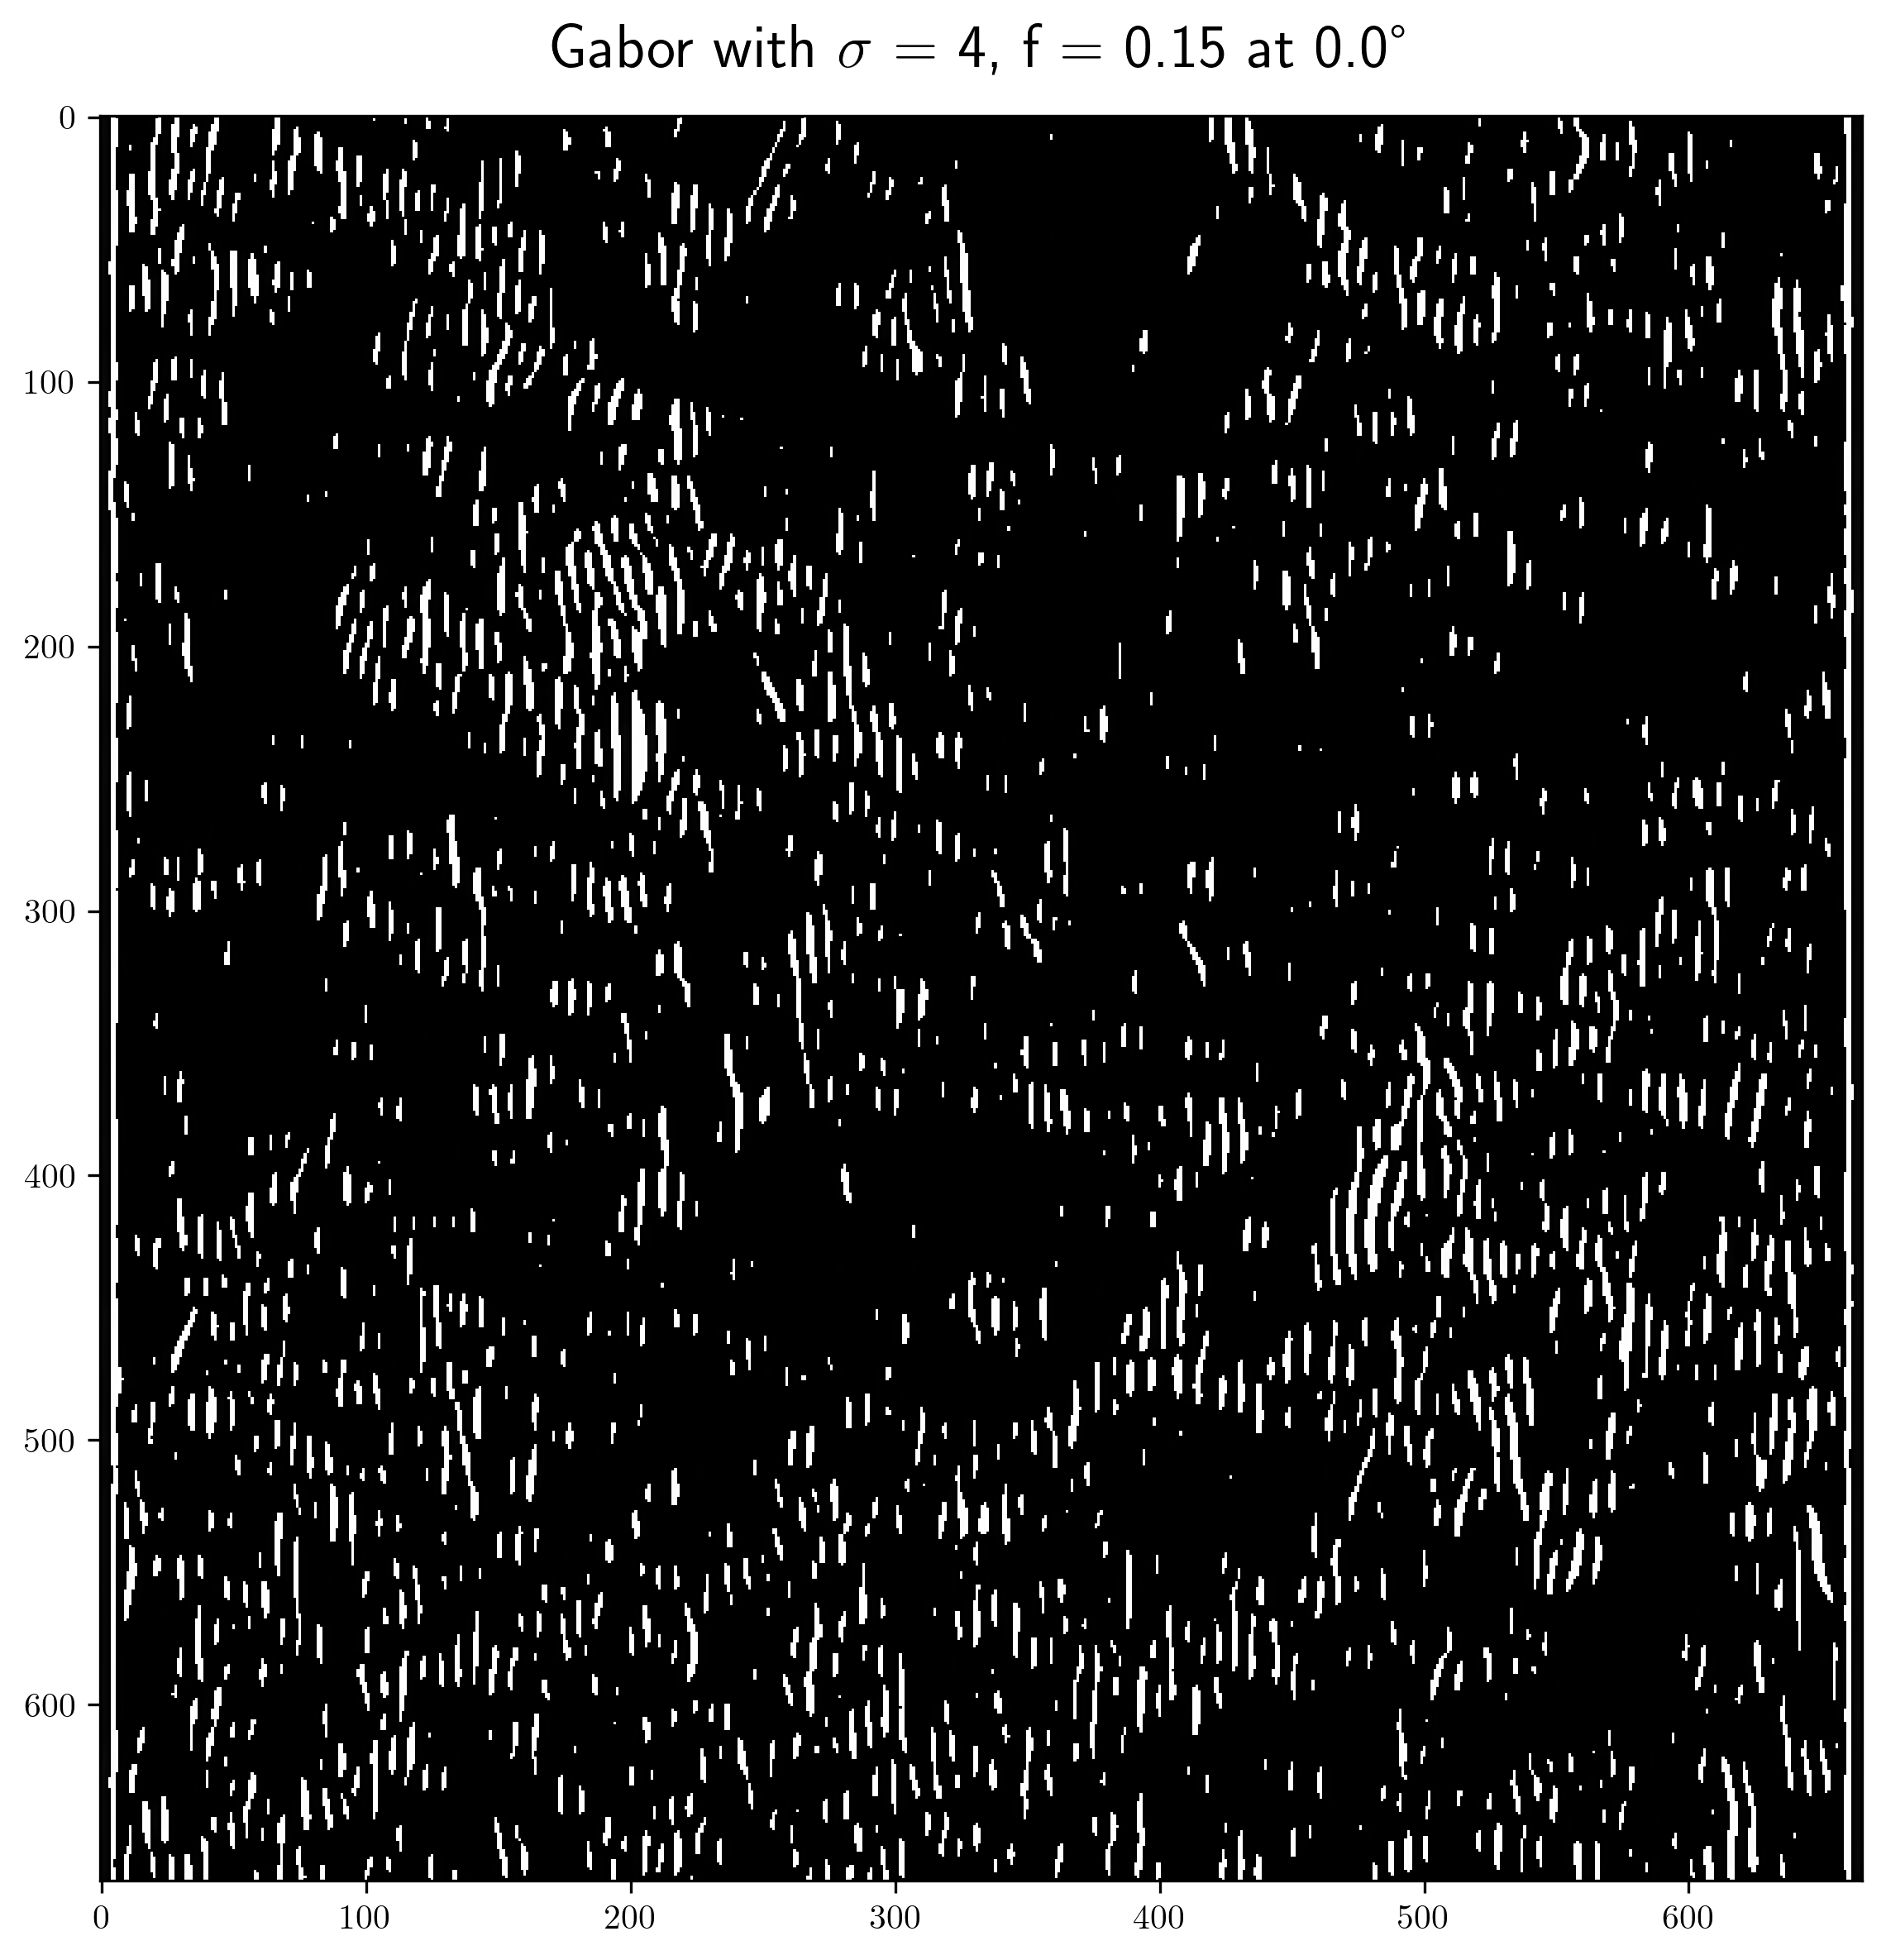
\includegraphics[width=\textwidth]{img/Features_4_015_0.png}
         \caption{Kernel with $\sigma$ = 4, f = 0.15 and 0 ° rotation}\label{fig:feat06}
     \end{subfigure}
        \caption{Result of convolving differently oriented gabor wavelets with an Landsat-8 image of Bremen}\label{fig:gaborExample}
    \end{figure}
%
\newpage
 \subsection{K-Means Clustering}\label{sec:kmeans}
K-means clustering is an unsupervised learning algorithm that is used to partition $n$ observations into $k$ clusters. 
Each observation belongs to the cluster with the nearest mean, serving as a prototype of the cluster. 
This method has many applications in data mining, image processing, and pattern recognition.
The algorithm consists of three steps:
\begin{enumerate}
    \item \textbf{Initialization}: Choose $k$ initial centroids from the data points.
    \item \textbf{Assignment}: Assign each data point to the nearest centroid, forming $k$ clusters.
    \item \textbf{Update}: Recalculate the centroids as the mean of all data points in the cluster. 
\end{enumerate}
This process is repeated until a maximum number of iterations or minimal changes in centroids is reached.\cite{Sinaga2020}\\ % TODO read
Mathematically a set of observations $(x_1, x_2, \ldots, x_n)$, where each observation is a $d$-dimensional real vector.
K-means clustering aims to partition the $n$ observations into $k$ ($\leq n$) sets $S = \{S_1, S_2, \ldots, S_k\}$ so as to minimize the within-cluster sum of squares. \\
The objective is to find:
\begin{equation}
    \min_{S} \sum_{i=1}^{k} \sum_{x \in S_i} \| x - \mu_i \|^2
\end{equation}
where $\mu_i$ is the mean of points in $S_i$.
%
The K-Means clustering algorithm is used for surface classification using the feature enriched multi band satellite data.
\Cref{fig:kmeansclusters} shows the result of clustering land surface types (the shown clustering did not use feature enhancement with Gabor and only used the band information as basis).%TODO fix that!  
    \begin{figure}[!htbp]
      \centering
      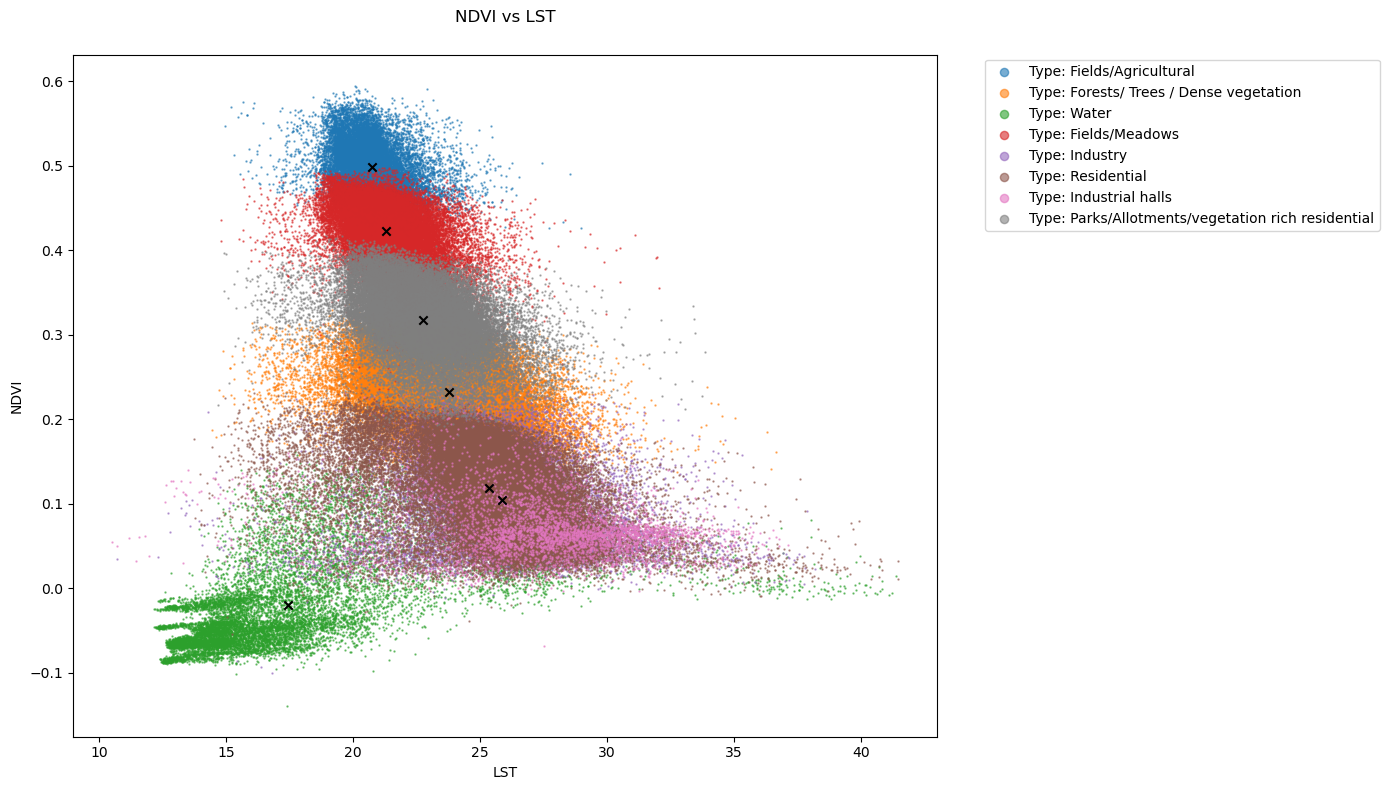
\includegraphics[width=\textwidth]{img/NDVI vs LST.png}
      \caption{Result of clustering (colored dots) plotted as \gls{NDVI} value and \gls{LST}\label{fig:kmeansclusters}}
    \end{figure}

 \subsection{Random Forrest Algorithm}\label{sec:randomForrest}
Random Forest is a versatile ensemble learning method widely used in machine learning for both classification and regression tasks.
It operates by constructing multiple decision trees during the training phase and outputting the mode of the classes (in classification) or mean prediction (in regression) of the individual trees.
This method is particularly noted for its robustness and ability to handle large datasets with complex structures.

The algorithm involves creating multiple decision trees using bootstrap aggregating, where each tree is trained on a random subset of the data with replacement, and at each node, a random subset of features is chosen for splitting.
The ensemble approach mitigates the risk of overfitting, a common problem in individual decision trees, making Random Forest an effective tool even in scenarios with noisy or incomplete data. 
In the Land Cover use case, this should increase robustness against seasonal variability of surface type appeal and changes due to variation in local climate and geology.\\ \\

One of the strengths of Random Forest lies in its capacity to provides a measure of feature importance, which is valuable for understanding the driving factors in a model and provides a point for further optimization in case the performance is not sufficient.
The downsides of the algorithm is, that it is computationally intensive, especially with a large number of trees, and the resultant model can be less interpretable compared to simpler models like linear regression or single decision trees.\\

In practical applications, Random Forest has been employed across various domains, ranging from predictive analytics in finance (e.g.\ in~\cite{Zhang2022}) and healthcare (e.g.~\cite{Kane2014}) and natural language processing. 
It is suitable for usage in time line analysis and was used in this application for predicting the surface types based on the imagery which has been show to be effective in the past in~\cite{Piao2021}.
%
Its ability to provide robust and accurate predictions even in the presence of complex data interactions has cemented its place as a staple algorithm in the machine learning toolkit.

\newpage
\section{Comparable Definition of Urban Heat Islands}\label{sec:definition}
    \subsection{Introduction}
    The definitions of \glspl{UHI} in the literature are varying slightly and do not take into account that, using remote sensing techniques most definitions do not allow easy comparison between different areas or times.
    Local studies either used a single reference measurement station %(TODO ) 
    or the surface temperature of surrounding rural areas like forests % (e.g.TODO add sources, maybe add examples? 
    The definition of the U.S.~EPA\cite{EPA2008} and the German Weather Service (\gls{DWD}) both say it is an feature defined by increased temperature between the urbanized areas compared to the sourrounding. % TODO cite  
    Different studies analyzing \glspl{UHI} use difference referenece tempereatures.
    The first goal of this work is defining a systematic reproducable aproach to measure urban heat island intensity.
%
    \subsection{Approach}
    To make the comparable, the method of~\cite{Sobrino2020} was adapted, where \gls{SUHI} where compared in different cities around the world using Sentinel-3 images.
    In that work a buffer zone was calculated around a citie and this was used to identify and measure the intensity of the heat islands within the city area.\\ 
    This work uses the same basic approach but Landsat 8/9 data was used and combined with different \gls{ML} techniques for surface classification (see \cref{sec:classification}). % TODO 
    In~\cite{Sobrino2020} urban adjacent, future urban adjacent and peri-urban areas are defined as buffers.
    These where adapted by removing the urban growth projection (since the scope of the paper was the investigation of \glspl{SUHI} in 2050 that does not match the goal for this work).
    The urban area is identified by detecting land cover classes indicating a larger area of build up classes. 
    These Areas are then converted into polygons that are extended by buffer zones as shown in \cref{fig:bufferedBremen}.
    \begin{figure}
      \includesvg[width=\textwidth]{img/UrbanAreaBremen}
      \caption{Urban Area of Bremen, with buffer zones for Adjacent and Peri Urban Area\label{fig:bufferedBremen}}
    \end{figure}
%    
    \subsubsection{Used Satellites}
    Using remote sensing data to detect and analyse \gls{SUHI} requires devices that are able to detect thermal infrared radiation. 
    Satellites that are equipped with thermal infrared sensors that are able to detect upwelling emission from the surface temperature within the $ 8 < \lambda < 12 \mu m $ range. 
    Instruments that were previously used for measuring \glspl{UHI} are Landsat, MODIS, ASTER and Sentinel-3. 
    In the following steps data from the Landsat 8 and Landsat 9 satellites was used, as well as Landsat 7 satellites images for historical data from before the launch of Landsat 8. 
    % TODO ref to or add landsat data description

    \subsection{Definition of Urban Heat Islands}\label{sec:definition}
    The Urban Heat Island is defined as an area with higher temperature.
    For comparability this should be a statistical metric that is based on the temperature ranges observed in the image.\\ 
    The proposed metric is that a heat island is an area that has a temperature that is at least two standard deviations above the average temperature of the sourrounding urban area. 
    The reference measurement is done using the surface temperature of the peri urban buffer zone and removing all larger urban areas within it. 
    This will get rid of other cities or larger industrial sides close to the area of interest.
    The mean temperature and variation within the peri urban area is then calculated and used as reference.
    % Assuming that temperature is normal distributed the temperature should lie outside of the 95%ile 
    Depending on season the temperature distribution will vary, due to the definition using the standard deviation the detection of urban heat islands is coupled to the range of temperatures observed within the image. 
    During processing single outlier areas as well as clouds, cloud shadows are removed and holes within the urban area are closed, this allows to include parks and other urban green areas to be processed and only includes larger areas of elevated temperatures as urban heat islands. 
    This will increase robustness of \gls{UHI} detection to reduce the influence of hot surfaces (such as solar panels or industrial tanks) during detection.
    % TODO normal dist? 
    
   TODO IMAGES for each step / marked with temps to make it easier to understand  

    \subsection{Conclusions}	
    The suggested approach proposes to use a statistical definition of Urban Heat Island, to be an area that is more then $2\sigma$ above the mean temperature of the surrounding area, while the sourrounding area is defined as a fixed buffer based on the size of the urban area and clean the area of larger settlements. 

%    
\newpage
\section{Impact of Land Cover Changes on Urban Heat Islands}\label{sec:LULC}
    \subsection{Introduction}
  One of the key factors influencing the intensity and distribution of UHIs is land cover change, primarily driven by urbanization and associated human activities.
    Soil properties impact the emissivity, thermal conductivity and heat capacity of an area and increases in build up reduce surface water availability. 
\\    
This section looks into the relationship between land cover change and UHI effects using LULC detection based on the previously classified Landsat images.
The exploration begins with an overview of the impact of land cover changes and the underlying mechanisms on Urban heat islands and highlighting the critical role that changes in land cover play in modulating urban thermal environments.
The discussion extends to the various types of land cover alterations, such as the replacement of natural landscapes with built-up areas, deforestation, and changes in vegetation cover, and how these modifications contribute to the exacerbation or mitigation of UHIs.
\\
Furthermore, the chapter examines the multi-dimensional impact of UHIs under the lens of land cover change.
This includes the analysis of spatial and temporal patterns of UHIs, the influence of different urban forms and structures, and the effectiveness of various mitigation strategies, such as urban greenery and reflective materials in buildings and pavements.
\\
Through a synthesis of current research findings and case studies, this chapter aims to provide a comprehensive understanding of the dynamics between land cover change and UHIs.
It also seeks to offer insights into sustainable urban planning and design practices that can mitigate the adverse effects of UHIs, thereby contributing to the development of more livable and resilient urban environments.
%
    \subsection{Impact of Land cover/ Surface type on Heat Buildup}
    %TODO 
    Todo literature recherche aus Obsidian einfügen... 
    %TODO 
    \subsection{Land cover classification}
	\subsubsection{Land Surface Temperature Calculation}\label{sec:lstcalc}
    The \gls{LST} can not be measured directly by a satellite but must be calculated from the upwelling thermal infrared radiation and corrected for the atmospheric perturbation. 
    For Landsat 7 and Landsat 8 data is provided in different processing levels.
    For analysis of past data that has already be processed the level 2 data can be used, that provides land surface temperature and has been calculated from the level 1 data. 
    The level 1 data provides \gls{TOA} brightness and is corrected for stray light (Landsat 8 specific, see~\cite[p.~67]{Zanter2019}) instrument distortion, geometric and geographic terrain-correction (\cite[p.~44]{Zanter2019}).
    The \gls{TOA} tempreature data is calculated according to \cref{equ:toa} where $K_1$ and $K_2$ are band specific conversion factors from the meta data file and $L_\lambda$ is the spectral radiance at the TOA in $\frac{W}{m^2\cdot srad \cdot \mu m}$ e.g.\ the Band 10 Channel. 
    \begin{equation}\label{equ:toa}
	    T = \frac{K_2}{\ln\left(\frac{K_1}{L_{\lambda}}+1\right)}
    \end{equation}
    % TODO This value is then corrected for emmissivity of the ground .... 
 
    The temperature is corrected for atmospheric interference using local reference stations and emmissivity using the global emmissivity database.  % TODO link 
    The USGS uses reference stations, atmospheric models and independent reference measurments from other satellites to calculate the Surface temperature, the surface temperature product has an accuracy of $\pm 1 K$ overall and other uncertainties are marked in a quality assurence file provided for each image.
    % TODO formula 
    \subsubsection{Classification }\label{sec:classification}
    The methodology employed for land cover classification involved the multi-step process utilizing satellite imagery, feature enhancement and machine learning techniques shown in \cref{fig:pipeline} and described in \cref{sec:pipeline}.
    The primary data source was 11-band Landsat images, which provided a comprehensive spectral view of the area to be classified.
    To augment the dataset and enhance the classification accuracy, Gabor filtering was applied to the Landsat images (as detailed in \cref{sec:gabor}).
    For classifying surfaces a mixed approach of clustering and unsupervised machine learning was used. 
    As input, the multispectral data from Landsat where used.
    The multi band image was loaded and cut to match one of the used training areas (%TODO ref picture
). 

    Each band of the image was then processed using a Gabor Feature Extraction algorithm (s. \cref{sec:gabor}) with different parameter sets. 
    It was found, by variation of parameters, that the highest score was archived using XXX 
%TODO try 
    rotations of the kernel, a kernel size of XXX
%TODO find 
    and (only circular kernel where used) with a $\lambda$ of 2 and 4. %TODO check 
    The frequencies of the sine wave where varied between 0.05 and 0.15. \\ 
    After the features were added the data was passed through the trained (random forest model \cref{sec:randomForrest}) for classification. 

This step was crucial in extracting and emphasizing spatial patterns and textures, thereby facilitating more distinct classification of land cover types. %TODO citation?
The classified image has 11 classes that are shown in \cref{tab:land_cover_classes}
\\
The feature enhanced data of images of Bremen%, Valencia and TODO 
were used of multiple years to create an unsupervised K-Means clustering model.%TODO add more 
This initial clustering served as the foundation for the subsequent Random Forest machine learning model.
The K-means algorithm was executed with varying numbers of classes – specifically 8, 10, and 11 – to determine the optimal classification schema.
This model was validated using the Sentinel-2 10m Land Use/Land Cover map (\cite{Zhang}).
Since the data set only uses 8 classes, the used classes where mapped to the best fitting class (indicated in \cref{tab:land_cover_classes}). 
Clouds, Cloudshadows and Snow/Ice where not used for verification and removed for the analysis.
%TODO
To judge results the output of the kmeans and the random forrest was compared to the ESA CCI Land Use Data Set~\cite{landformclassicationusingfuzzykmeans2000} that was scaled up to the used image resolution. %TODO check if correct reference
\\
TODO THE VALIDATION RESULTS STILL TBD... :/ 
\\ 
The Trained model was then used to classify other cities and datasets from different times. 
Part of the training data as well as different time data from the same area was used and Feature enhanced using the same Gabor-Filter bank.
Feeding the enhanced data into the random forests model was then used to determine the land cover classes for the next step of the analysis.
\begin{table}[h]
\centering
\caption{Land Cover Classes Identified\label{tab:land_cover_classes}}
\begin{tabular}{lp{4cm}l}
\toprule
\textbf{Class Number} & \textbf{Land Cover Type} & \textbf{ESRI Class}\\
\midrule
1 &  Allotments and vegetation rich residential area  & Build Area\\
2 &  Industry Halls & Build Area\\
3 &  Forest and dense vegetation& Trees \& Crops\\
4 &  Agricultural Land & Crops\\
5 &  Water& Water / Flooded Vegetation\\
6 &  Industrial& Build Area\\
7 &  Bare Soil, Rock & Bare \\
8 &  Cloud Shadows & Clouds \& Any \\
9 &  Fields and meadows& Rangeland \&Crops \\
10 &  Clouds & Clouds \\
11 &  Residential/ Build-up& Build Area\\
\bottomrule
\end{tabular}
\end{table}
For the labeling of these land cover classes, the Normalized Difference Vegetation Index (NDVI) and the Normalized Difference Built-up Index (NDBI) bands were utilized.
These indices were instrumental in differentiating vegetated areas from built-up regions, thereby aiding in the accurate categorization of land cover types.
The classification labels were assigned based on the proximity of the NDVI and NDBI values to the cluster centers derived from the K-means model.
This approach ensured that each land cover class was consistently labelled independent of the study area.\\
%
\subsubsection{Urban Area Extraction}
    The resulting classified image was then processed to extract urban areas.
    The algorithm used the classes 1,2,6 and 11 from \cref{tab:land_cover_classes} to detect areas that can be considered urban.
    The areas were \gls{dilated} and \gls{eroded} to bringe small gaps between parts of the citie and close holes as well cut small links such as highways between areas.
    After this preprocessing step the areas are enumerated and all areas that cover at least 1\% of the image area where used to create buffer zones. 

    Bufferzones where defined as: 
    \begin{equation}
	    W_U = \frac{A_U^{\frac{1}{2}}}{4}
	    W_P = \frac{6\cdot A_U^{\frac{1}{2}-W_U}}{4}
    \end{equation}
    Where $W_U$ is the Urban and Suburban area (the urban area and a suburban buffer zone) and $W_P$ the peri urban area.
    These definitions where used in~\cite{Sobrino2020} and were developped in the 90s for urban development (\cite{AlkanBala2014}).
   \\ 
\\
    TODO add images or code snippet



 \subsection{Analysis}\label{sec:landcoverAnalysis}
TODO Daten einfügen und analyse ergebnisse
  \subsection{Conclusions}
In summary, the integration of enhanced Landsat imagery, Gabor filtering, K-means clustering, and Random Forest classification constituted a robust methodology for land cover classification.
This process not only facilitated a detailed and accurate representation of the study area's land cover but also demonstrated the efficacy of combining various remote sensing and machine learning techniques for environmental analysis.
TODO nochmal etwas genauer beschreiben. ADD DATEN und Bilder! 
%
\newpage

  \section{Impact of Climate Change on Urban Heat Islands}\label{sec:UHITempImp}
    \subsection{Introduction}
    The interaction between global and local climate is a complicated process that has multiple parameters, that are not completely understood nor are they all easily measurable. 
    In central Europe the climate is governed by seasonality typical for the northern hemisphere.  
    According to multiple studies global rise of temperature due to climate change is also increasing temperatures in northern Europe~\cite{Benestad2005}  %TODO this is not really what I want...

    %A climate tipping point (see~\cite{Lenton2008}) that could cause severe cooling in northern Europe is the breakdown of the Atlantic Thermohaline circulation\cite{Rahmstorf1999}.
    %TODO add a sentence for why
    %But since the European climate is still under influence by the warm ocean currents, 
    The temperatures in major European cities have increased at a similar pace then the global mean temperatures. 
    The cities covered by this study observed an average increase from 1990 to 2020 of %TODO 
    \textdegree\ C. 
%
    The hypothesis is that the rising temperatures observed over the past 30 years have increased heat island severity and size. 
    \subsection{Methodology}
    Measurement of the impact on rising temperatures have to be done after correcting for other variables such as urban development, meteorological impact factors such as wind and rain. 
    To archive this a time series of land surface temperatures and urban heat islands from 1990 to 2022 was created using Landsat 7 and Landsat 8 and 9 data.
    Data from weather stations in the areas where used to calculate the trend of mean temperature over the time. 
    The \glspl{UHI} data was then correlated with the air temperature data of the local measurement stations and corrected for size increases of urban heat island impacted by land cover change in the previous step. 
    This way in the statistical analysis all \glspl{UHI} that would be impacted by urbanisation or change of surface type where excluded from the analysis.
%
    %\subsection{Analysis}
    %\subsection{Conclusions}{sec:conclusion}
%    \section{Simulation and Modeling of \texorpdfstring{\glsxtrlongpl{UHI}}{Urban Heat Islands}}\label{sec:modelling}
%    \subsection{Introduction}
%
%    \subsection{Analysis}
%    \subsection{Conclusions}
%\newpage
%\section{Discussion}\label{sec:discussion}
%    \subsection{Synthesis of Findings}
%    \subsection{Implications}
%
\section{Conclusion}\label{sec:conclusion}
\subsection{Summary}
% Summary of the findings 
% contributions to research

\subsection{Limitations and Challenges}
% Why was something not possible
While the connection of ground based sensor stations with remote imagery works well, a direct reliable calculation 
% 
\subsection{Future Work}

\newpage
\section{Appendix}
%    \subsection{Data}
%    \subsection{Code}
%
%
\newpage
\printbibliography%
\newpage
\section*{Eigenständigkeitserklärung}

  % TODO insert Eigenständigkeitserklärung
\end{document}

%The surface classes where correlated with the %TODO check 
%Kataster data from Bremen as well as with OSM data. % todo do 
%
%Ziel Projekt teil: 
%- detection and error margins in UHI detection using remote sensing data 
%- data pipeline to create maps of UHI in areas 
%- surface classification based on remote sensing data correlated with 2nd and 3rd sources (kataster/ OSM) 
%- UHI "cores" identification 
%
%Master Fragestellungen: 
%- Correlation zw. UHI} und Pollutants? 
%https://pubs.acs.org/doi/epdf/10.1021/cr5006815 
%- Real time UHI size/occurrence prediction based on ground temperature stations (Bremen Airport) and pollutant levels? 
%- UHI classification in different environments, causes and effects, mitigation stategies? (e.g. Classification of Surface types, vegetation etc. within different climate zones (Phoenix, Bremen, Karlruhe, Essen, Something meditareiean, Afrika (coastal, arid, etc) /paper with adis abbeba)
%
%\subsection{}

%Of the different bands available from the used satellite data (Landsat7 and Landsat8), 
%the visible and near infrared bands where used for clustering. 
%The clustering was done using the simple k-means algorithm. 
%Different configuration where used %todo add pictures? 
%These where compared and referenced with ground truth data %todo add error and limitations refgerenec here 


